%Chapter 2: Seismogeodesy and Strong Motion Sensing

\chapter{Seismogeodesy}

Sesimic and geodetic networks for observation of earthquakes at regional distances (a few hundred kilometers) have developed mostly independently over the last few decades. it is unsurprising then that the different sensors types are infrequently collocated. Throughout this chapter we will discuss and demonstrate how both kinds of sensors can make important contributions to the characterization of strong ground motions. We will show that the shortcomings of one instrument can be alleviated by considering the other kind. We will propose and demonstrate a Kalman filter algorithm that can combine seismic and geodetic data in real time. As a consequence of our analysis we will conclude that if a seismic (or geodetic) network requires the computation of broadband strong motion displacement and velocity waveforms as part of its observational goals then priority should be given to the collocation of instruments and the combination of data sets

\section{Background on Strong Motion Sensing}
\label{sec:strongmotion}

The range of motions produced by the seismic source is broad both in frequency and dynamic range. It is well known that no one sensor can capture all signals of interest to seismology and earthquake engineering \citep{Havskov2006}. Seismologists typically rely on inertial sensors, seismometers, whose response is related to velocity of the ground, for measurement of small amplitude signals (weak motion). For large amplitude signals these sensitive instruments mechanically clip. In such a case, strong motion sensors, whose response is related to the acceleration of the ground and have lower gains, are preferred. Modern observatory grade accelerometers rely on the force feedback principle and can measure motions as small as 1nm at 1Hz and 100nm at 0.1Hz and accelerations of up to 4g. Furthermore their frequency response is flat from 0Hz (often called the DC-level) to 50-200Hz \citep{Havskov2006}.

Thus, in principle there should be no difficulty in integrating a strong motion record to velocity and displacement. This is not the case; in practice the simple integration of an accelerogram produces unphysical velocity and displacement waveforms that grow unbounded as time progresses. Computation of broadband displacements from strong motion recordings is a thoroughly studied procedure that is fraught with many known problems and has no known single solution. By ``broadband displacement'' we mean a strong motion displacement waveform that captures both transient or dynamic phenomena (waves) and permanent or static deformation, i.e. a recording reliable from DC to the Nyquist frequency.

The problems associated with the double integration of accelerometer recordings have been comprehensively studied and many sources of error have been suggested: numerical error in the integration procedure, mechanical hysteresis, cross-axis sensitivity and unresolved rotational motions \citep{Graizer1979,Iwan1985,Boore1999,Boore2001,Boore2002,Smyth2007}. It is generally assumed that as a consequence of one of the afore mentioned problems small offsets are introduced in the acceleration time series; upon integration these \textit{baseline offsets} produce the linear and quadratic trends observed in the velocity and displacement time series, respectively. Of the possible sources of these offsets unresolved rotational motion is often invoked as the main error \citep{Graizer2006,Pillet2007}. Motion is described by six degrees of freedom, three translations and three rotations. Accelerometers, as inertial sensors, are incapable of discerning between rotational and translational motions, thus, rotational motions are recorded as spurious translations. Effectively, this results in a change of the baseline of the accelerometer, even if by a small amount, leading to unphysical drifts in the singly-integrated velocity waveforms and doubly-integrated displacement waveforms (Figure \ref{fig_iwt009}).

\begin{figure}[!ht] 
  \centering
  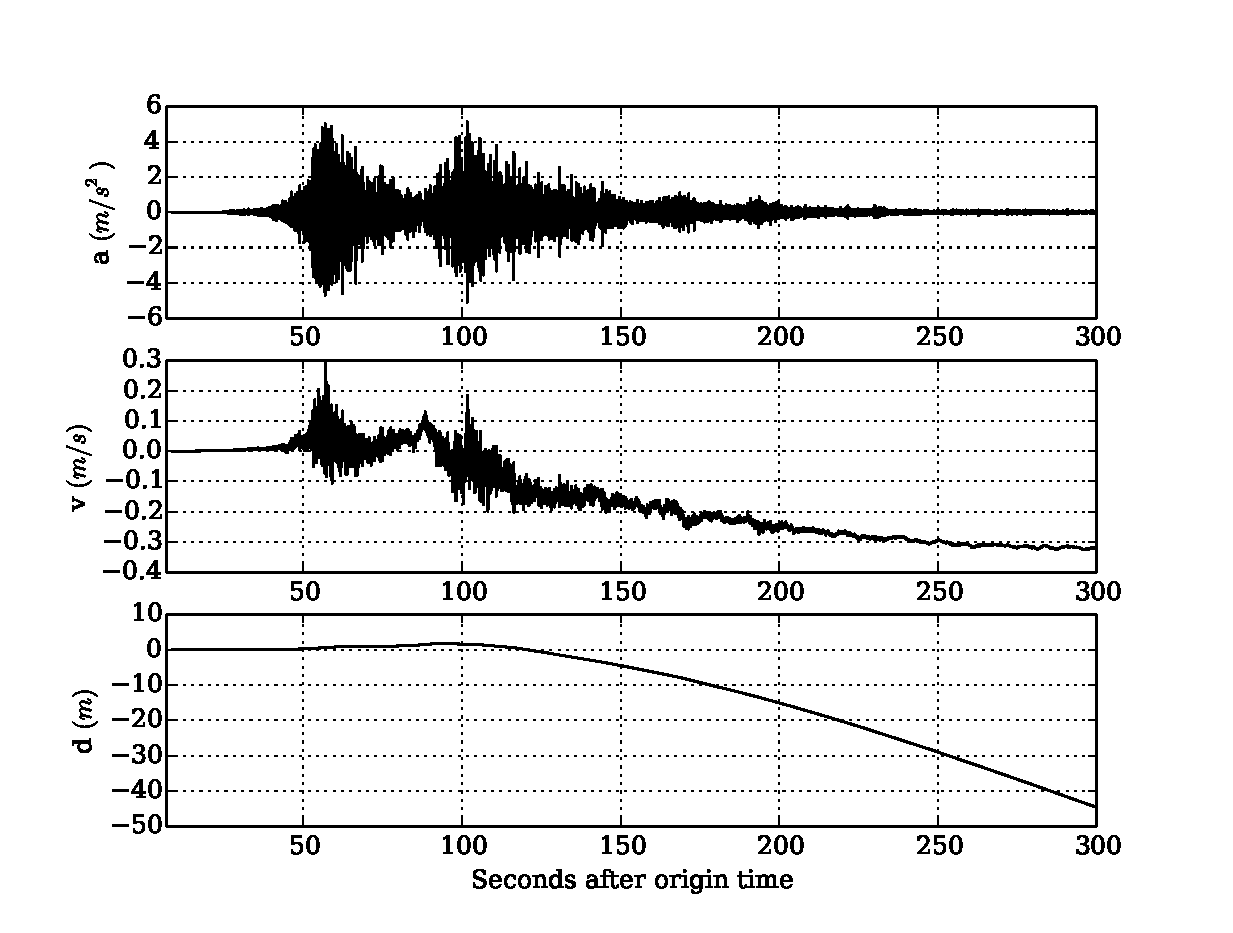
\includegraphics[width=0.99\linewidth]{./figures/ch2/iwt009.eps}
    \caption[Effect of numerical integration on a strong motion recording.]{Effect of numerical integration on a strong motion accelerogram. This example is for the east component of motion at station IWT009 192 km from the centroid of the 2011 $M_w$9 Tohoku-oki earthquake. Note the unphysical drifts in both the velocity and displacement time series.}
  \label{fig_iwt009}
\end{figure}

Many correction schemes, collectively known as baseline corrections, have been proposed over time to deal with this problem. Rotational motions become more prevalent close to the source and at long periods. In particular, \citet{Trifunac2001} have shown that rotational motions have significant contributions to radiated spectra and can sometimes be the predominant source of seismic energy, particularly at very long periods and for very large earthquakes. 

For this reason, the simplest baseline correction scheme is a high-pass filter \citep{Boore2005}, eliminating the baseline-shifted long period portion of the time series. This leads to accurate recovery of the mid to high frequency part of the displacement record but suppresses completely low frequency information such as the static offset (Figure \ref{fig_iwt009bl}). To ameliorate this, a number of more elaborate correction schemes exist \citep{Boore2005} that rely on function fitting to the singly integrated velocity time series. The most reliable scheme that routinely produces plausible displacement waveforms (which include a measure of the static offset) is described in \citet{Boore1999, Boore2001} and is a modification of the scheme proposed by \citet{Iwan1985} and henceforth referred to as the Boore-Iwan or BI correction scheme. In this method a piece-wise linear function is fit to the uncorrected velocity time series, the slope of each straight line segment represents an acceleration step which is then subtracted from the original acceleration data. This baseline corrected acceleration record is subsequently integrated to velocity and displacement. If the intervals for fitting the linear functions to the velocity data are selected appropriately this algorithm will produce waveforms that look plausible. They will contain both permanent and transient motions. The difficulty then lies in determining what these appropriate time intervals are from the data themselves. As discussed by \citet{Boore1999,Boore2001} this is an ambiguous process. To diminish this uncertainty, subsequent research has focused on determining plausible times for the fits and then grid searching for waveforms that most resembles a ramp or step function \citep{Wu2007,Chao2010,Wang2011}.

\begin{figure}[!ht] 
  \centering
  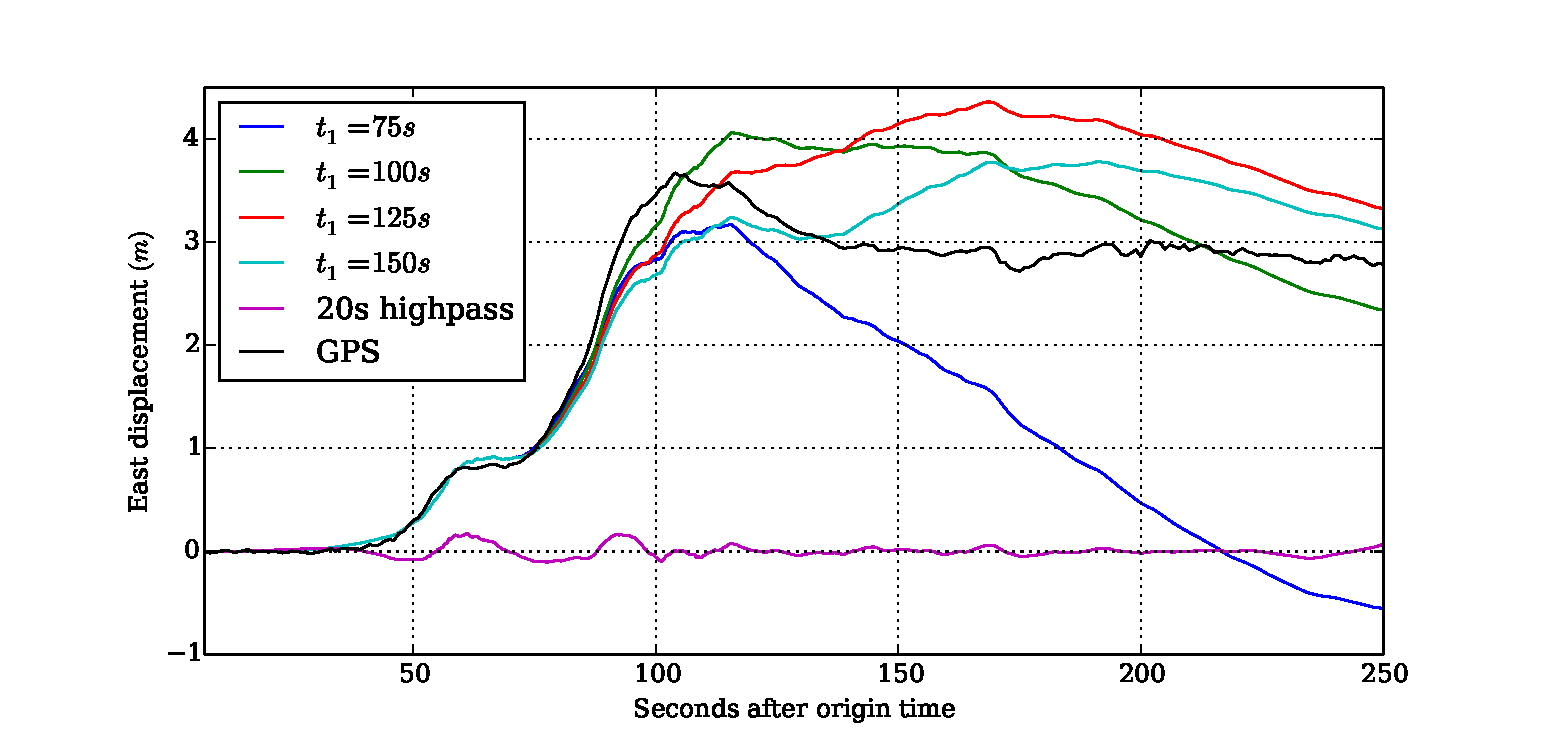
\includegraphics[width=0.99\linewidth]{./figures/ch2/iwt009bl.eps}
    \caption[Some simple baseline corrections.]{Baseline corrections using the BI algorithm for the east component of motion at station IWT009 192 km from the centroid of the 2011 $M_w$9 Tohoku-oki earthquake using different values of the correction parameter $t_1$. Also shown is the result of a 20s high pass filter corrected waveform and the GPS displacements recorded at the same site}
  \label{fig_iwt009bl}
\end{figure}

This is better understood through an example. Consider the time series of Figure \ref{fig_iwt009}. The traditional BI correction procedure starts by removing the pre-event mean or baseline, this is called the zeroth-order corrected waveform. Then for some analyst-determined initial correction time $t_i$ and final correction time $t_f$, two baselines, or acceleration steps, can be computed from the drift in the velocity data and subsequently removed. Underlying this process is the assumption that from time $t_i$ to some intermediate time $t_1$ (determined by the analyst) a baseline offset due to strong shaking is introduced into the time series and subsequently from this intermediate time $t_1$ to the final correction time $t_f$ a permanent baseline offset is introduced into the data. Thus, the first acceleration step is determined by a least squares straight line fit to the velocity data between times $t_1$ and $t_f$ such that
\begin{equation}
v_f(t)=v_0+a_f(t)\;;\;t\in(t_1,t_f)\;,
\end{equation}
where the regression parameters are $v_0$ and the acceleration step $a_f$. Subsequently, another straight line is fit from $t_i$ to $t_1$ with the constrain that velocity be zero at the start of the record and that the final velocity averages to zero. These constraints are satisfied if \citep{Boore1999}
\begin{equation}
a_m=\frac{v_f(t_1)}{t_1-t_i}\;.
\end{equation}
Then, the acceleration baseline, $a_m$, is subtracted from the uncorrected record from times $t_i$ to $t_1$ and the baseline offset, $a_f$, is subtracted from the zeroth order corrected record for times $t_1$ to $t_f$. The record is then integrated to velocity and displacement. This scheme produces waveforms that look plausible; they contain both transient and permanent motions. However an ambiguity lies in the selection of times $t_i$ and $t_1$. As has been amply discussed by \citet{Boore1999,Boore2001}, this ambiguity is not easily resolved without external information and each investigator relies on subjective judgment to ascertain what looks best. Figure \ref{fig_iwt009bl} illustrates such an example where the same waveform has been baseline corrected for several values of $t_1$ while holding $t_i$ fixed at the \textit{P} wave arrival time with results that vary wildly. If the waveform is complex, as in this example, with two distinct pulses of very strong shaking, then more baselines might need to be subtracted. However, if there is already ample ambiguity in the simple determination of the two baselines $a_m$ and $a_f$, the problem is exacerbated with the introduction of more baselines. 

The correction times $t_i$ and $t_1$ can and do vary for each station-event pair and even for different channels at the same station during the same event. Practically this means that analysis of broadband displacements from baseline-corrected accelerometer records is inherently ambiguous and complicated for real-time seismological applications or across large networks both for real-time and post-processing purposes.

Research into automated baseline correction from accelerometer data alone has focused on variations of the BI scheme. \citet{Wu2007} proposed a variant in which the times for each linear segment of the baseline correction are determined by a grid search such that the resulting time series best matches a ramp function. \citet{Chao2010} elaborated on the formulation of \citet{Wu2007} by adding an extra restriction that the times be selected after certain threshold values of acceleration energy have been accrued. Both studies compared their results to static offsets determined from GPS and found that their estimates are somewhat similar. There is still scatter in he comparison between the static field derived front he corrected data and that determined from nearby GPS. Additionally, no analysis on the adequacy of the remaining part of the waveform is performed. It is implicitly assumed that if the static field is well fit then the rest of the waveform will be reliable as well.

An important advance in automatic baseline correction is presented in \citet{Wang2011} who present another variation of the BI bilinear scheme that performs better than those discussed thus far. They developed some simple heuristics for determination of the interval of possible correction times based on analysis of the uncorrected acceleration and displacement waveforms. From an analysis of the time at which the peak ground acceleration (PGA) occurs and the time of last zero crossing in the uncorrected displacement they determine bounds for the grid search of baseline correction times. They then perform the grid search among these possible correction times and fit, via a non-linear regression, a step function to all possible waveforms. An optimum correction (the one that best fits this step function) is then selected. Unlike previous studies they compare their results not only to measured static offsets but to observed 1Hz GPS data; they do this for a single station. They find for that one station an error of $\sim$20\% in the static field estimation but a very good agreement between the corrected displacement and the GPS for the first 200s of the waveform.

In a follow up study \citet{Wang2013} apply their methodology to accelerometer records for the 2011 $M_w$9.0 Tohoku-oki earthquake. They obtain reasonable estimates of the static field for many stations in the KiK-net network in Japan but also find numerous outliers. They then develop a simplified scheme to screen the outliers by excluding coseismic offsets that deviate more than 15$^\circ$ from the predictions of a static slip inversion. Furthermore, they compare their automatic corrections for selected borehole sensors in the KiK-net network with nearby high-rate GPS stations with mixed results. They find that while parts of the waveforms might be a good match, the static estimates can be in error by a significant amount. To ameliorate this they then propose to use the static field from nearby GPS stations as a constrain in the correction procedure. From the pool of all candidate baseline corrections they select the one that fits a step function of amplitude given by the static field. In a follow up study \citet{tu2014} showed that substantial improvement was possible if corrections were correlated between neighboring stations of a dense network. It is noteworthy that \citet{Wang2013} and \citet{tu2014} and  do not provide baseline corrected solutions for the sister strong motion network K-net. They readily acknowledge that K-net stations, which generally have less favorable site responses \citep{tsuda2006}, are not well modeled by this automatic approach. This will be important later on in this chapter when it is shown that K-net data can be corrected as well as KiK-net data. In general while these algorithms have demonstrated incremental improvements to the original BI correction scheme they are far from being routinely applicable, objective or automatable.

The availability of suitable correction algorithms for strong motion waveforms that can produce broadband displacements is of broad interest especially for source analysis and hazards assessment. There has been ample interest in recent years to access to such real-time broadband displacements. Recall that it is the long periods of the seismic spectrum down to the static offset that provide the most obvious demarcation between large events. Static offsets and long period radiation can be used to rapidly compute moment tensors, source dimensions, static and kinematic source models and tsunami models. Indeed in Chapters 3,4 and 5 we will show how broadband strong motion waveforms facilitate such computations.

\section{The Role of GPS}
\label{sec:gps}

An alternative to baseline corrections of strong motion data is to measure displacements directly using the  Global Positioning System (GPS). There are two basic approaches to precise GPS data analysis: network positioning and precise poin positioning (PPP). In both approaches stations positions are estimated with respect to a global Cartesian terrestrial reference system. This system is realized by the published coordinates and velocities of hundreds of global geodetic stations in the International Terrestrial Reference Frame (ITRF). Precise GPS satellite orbital products distributed by the International GNSS Service (IGS) are tied to this underlying reference frame, and without loss of generality, are assumed to be fixed in the GPS data analysis. 

In network positioning, data from a network of stations are analyzed simultaneously to estimate station positions and integer-cycle phase ambiguities \citep{Dong1989,Blewitt1989}, and other parameters such as zenith troposphere delays. Analyzing the data as a network, results in the effective cancellation of GPS receiver clock and satellite clock errors, which are common to multiple satellite and stations, respectively. Precise poin positioning \citep{Zumberge1997} relies on fixed satellite orbits, as well as satellite clock parameters also available through the IGS and/or its different analysis centers . These parameters are held fixed in the process of estimating ITRF positions of individual GPS stations, phase ambiguities, zenith troposphere delays and station clock parameters.

Network positioning and precise poin positioning approaches can be considered equivalent, in terms of the underlying physics. However, to achieve geodetic quality positions (mm- to cm-level), it is essential to resolve integer-cycle phase ambiguities to their correct integer values \citep{Blewitt1989,Dong1989}. This is straightforward for batch post-processing, which includes the simultaneous analysis of multiple GPS data records, usually sampled at rates of 15-30 s, to derive a single station position over the entire sampled interval. It is the source of the typical 24-hour GPS position time series used to study permanent deformation, including long-term tectonic motion, as well as coseismic, postseismic and other transient deformation. Batch post-processing plays a role in seismological applications by providing highly-accurate, true-of-date ITRF station positions with respect to which displacement waveforms can be estimated during an event. There are several analysis groups that are producing 24-hour position time series on an operational basis.

Of primary importance in seismological applications is the estimation of cm-level or better displacements at the GPS receiver sampling rate, typically 1Hz. Since the first pioneering efforts over a decade ago \citep{Nikolaidis2001,Larson2003,Bock2004,Miyazaki2004} post-processed single-epoch network positioning with resolution of integer-cycle phase ambiguities is now routinely applied to seismology.  However, a general real-time solution is still elusive, and analysis of multiple data epochs is usually required to resolve integer-cycle phase ambiguities and estimate single-epoch positions.

In the network positioning approach typically, and for computational efficiency, the larger network is divided into multiple subnetworks with a 2-station overlap between adjacent subnetworks, and positions are estimated relative to the true-of-date ITRF coordinates of an arbitrary station within each subnetwork. Then, a network adjustment is performed to estimate coordinates for all stations with respect to the true-of-date ITRF coordinates of one or more stations outside the zone of deformation \citep{Crowell2009} easily providing centimeter level resolution.

Precise poin positioning has been limited in GPS seismology, in particular for real-time applications, because of unresolved integer-cycle phase ambiguities and slow convergence rates and re-convergence rates when loss of lock on the satellite signals occurs. JPL'��s Global Differential GPS (GDGPS) System employs a large global ground network of real-time reference receivers and real-time data processing software, which allows a single GPS receiver to be poin positioned with 10-20 cm accuracy anywhere in the world. This level of accuracy is considered useful for global tsunami warning generated by great earthquakes. A relatively new area of geodetic research is rapid integer cycle ambiguity resolution in precise poin positioning (PP\textit{P} AR), without the need for specific reference stations. Besides fixed satellite orbits and clocks, and estimation of positions, receiver clocks and tropospheric delays of the GPS signals, it also requires prediction of ionospheric delays. Recent results have been encouraging in that reliable ambiguity resolution and cm-level positioning accuracies have been achieved with only a few epochs of 1Hz GPS data for re-convergence \citep{Geng2010}. It has since been shown with a study of modestly sized earthquakes (M5) during the 2013 Brawley swarm \citep{Geng2013} and shake table tests \citep{Geng2013b} that the PP\textit{P} AR method is evolving to a state were it can be considered viable technology for real-time and rapid position calculations with cm-level precision.

It is important for the reader to understand the benefits and shortcomings of these two competing technologies. The network adjusted positions have routinely provided cm-level waveforms \citep{Crowell2009}. However, they require that the base station for the adjustment be located outside the zone of deformation and that it not move during the event. Evidently this requires a large network with good connectivity and some strategy for detecting motions of the reference station and a fall back plan to another station that has not moved during the event. Furthermore this approach requires converting the baselines between stations in subnetworks or triangles into absolute motions. This is essentially a solution to an inverse problem at each epoch. While this is not numerically troublesome for modest networks as the number of stations increases and as sampling rates grow the numerical load will mount.  In contrast the PP\textit{P} AR approach does not require such a reference station (although it does rely on a sparse continental network for computation of certain positioning parameters, \citep{Geng2013} and is thus, in principle, more desirable. However ambiguity resolution might fail and re-convergence periods, at least initially, can still be long. Throughout this dissertation data from both network adjusted and PP\textit{P} AR positions will be employed. it is not the aim of this work to assess the suitability of one technique over the other although some general recommendations will be given in the conclusions. Hence for the purpose of the research discussed both approaches will be considered equal.

In general GPS seems desirable over traditional seismometry for displacement computations. it is not an inertial sensor and thus not affected by baseline offsets. This has the practical effect of making GPS a very good long and ultra-long period sensor. It can easily measure signals with very long periods, such as plate tectonic motions and post-seismic relaxation. Consider Figure \ref{fig_parkfield}, note how the time series shows the (relative) long term plate rate as a linear trend, the coseismic offset from the September 28, 2004 $M_w$=6.0 Parkfield earthquake and the postseismic relaxation as well as some shaking during the earthquake. GPS seamlessly captures most key components of the seismic cycle. 

\begin{figure}[!ht] 
  \centering
  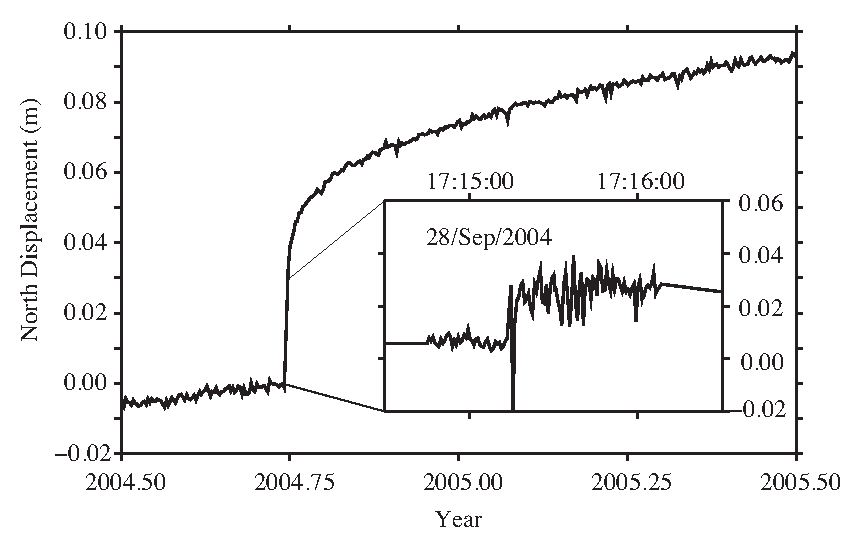
\includegraphics[width=0.99\linewidth]{./figures/ch2/parkfield.eps}
    \caption[1 Hz GPS time series at Parkfield]{Typical 1 Hz GPS raw time series at station LAND (35$^\circ$.8997 N, 120$^\circ$.4731 W) in the Parkfield area over a one-year period. Shown is the north component, in this case relative to station CRBT (N 35$^\circ$.7916, 120$^\circ$.7507 W) whose coordinates were fixed in the GPS analysis. Note how the time series shows the (relative) long term plate rate as a linear trend, the coseismic offset from the September 28, 2004 $M_w$=6.0 Parkfield earthquake and the postseismic relaxation. In the inset, 2 minutes of data are shown where as opposed to the daily solutions time series we can also observe the (relative) dynamic shaking during the earthquake.}
  \label{fig_parkfield}
\end{figure}

However, noise levels in high rate real-time GPS (rtGPS) displacements \citep{genrich2006} far exceed those of observatory grade accelerometers. Furthermore GPS data is far more verbose than seismic data. While a traditional telemetry packet for a seismic sensor at a given epoch might include three single or double precision floating poin numbers corresponding to the three components of motion and a UTC time string, the GPS message includes observables to every visible satellite. This has limited the sampling rates of rtGPS to around 1-5Hz even though 10-50Hz is achievable \citep{genrich2006}. These slow sampling rates can introduce significant aliasing in GPS positions \citep{smalley2009}. In spite of these limitations, it will be shown that without GPS positions it is exceedingly difficult to recover the long period component of ground motions and that GPS plays an important role in modern strong motion seismology.



\subsection{Displacements in a Local Reference Frame}

GPS positions are typically computed in a global reference frame (the International Terrestrial Reference Frame, ITRF) in what is known as Earth-centered Earth-fixed coordinates. This is a right handed system where the three Cartesian axes have an origin at the geocenter of the planet, one axis points towards the geodetic pole and two towards the equator. Without loss of generality or consideration for the particular GPS analysis technique used, or whether or not performed in real time or post processing, we assume that displacement waveforms are available for a geophysical event (e.g., earthquake) for one of more continuous GPS (CGPS) stations with centimeter-level or better single-epoch precision at, for example, the typical 1Hz sampling rate of current real-time geodetic networks. Consider that we know the precise coordinates $(x_0, y_0, z_0)$ of a CGPS station in a global Cartesian reference frame just prior to an earthquake, at time $t_0$. The prior coordinates represent ``true-of-date'' values. The station is then subjected to a combination of dynamic and static displacements. The subsequent coordinates of the station are denoted by $(x_i, y_i, z_i)$, where $i$ denotes the $i$-th epoch after the event. The displacement at the $i$-th epoch can be simply computed as $(x_i-x_0, y_i-y_0, z_i-z_0)$. In order to compare the geodetic displacements to displacements derived from a single integration of a seismometer or double integration of an accelerometer, we need to transform the displacements from a (right-handed) global Cartesian frame $(x,y,z)$ into a (left-handed) local North, East, Up frame $(N,E,U)$ by the following transformation
\begin{equation}
\label{eq_rot}
\left(\begin{array}{c}
\Delta N_i  \\
\Delta E_i  \\
\Delta U_i  
\end{array}
\right)
=
\left(
\begin{array}{ccc}
1 & 0 & 0 \\
0 & 1 & 0 \\
0 & 0 & 1  
\end{array}
\right)
\mathbf{R}_2\left(\frac{3\pi}{2}-\phi\right)\mathbf{R}_3(\lambda)
\left(
\begin{array}{c}
x_i-x_0 \\
y_i-y_0 \\
z_i-z_0  
\end{array}
\right)\;;
\end{equation}
where $\mathbf{R}_2$ and $\mathbf{R}_3$ are rotation matrices around the $y$ and $z$ axes, respectively, and $(\phi,\lambda)$ is the geodetic latitude and longitude of the station. The geodetic displacements in the $(N,E,U)$ frame can then be compared directly to local displacements derived through single integration of seismometer data or double integration of accelerometer data. Thus, Equation \ref{eq_rot} simplifies to:
\begin{equation}
\left(\begin{array}{c}
\Delta N_i  \\
\Delta E_i  \\
\Delta U_i  
\end{array}
\right)
=
\left(
\begin{array}{ccc}
-\sin{\phi}\cos{\lambda}  & \sin{\phi}\sin{\lambda}  & \cos{\phi}  \\
-\sin{\lambda}  & \cos{\lambda}  & 0  \\
\cos{\phi}\cos{\lambda}  & \cos{\phi}\cos{\lambda}  & \sin{\phi}   
\end{array}
\right)
\left(
\begin{array}{c}
x_i-x_0 \\
y_i-y_0 \\
z_i-z_0  
\end{array}
\right)\;.
\end{equation}

\section{Optimal Combination of Seismic and Geodetic Data}

As discussed in the previous section both traditional seismometry and GPS have advantages and disadvantages when it comes to sensing strong ground motions. GPS and strong motion networks are complementary in the sense that ones weakness can be complemented by anothers strengths. In particular GPS has slow sampling rates while accelerometers have fast sampling rates; in turn, accelerometers suffer from problems at long periods while GPS excels in this frequency band. Throughout this section we will show that the combination of these two sensor types provides an accurate representation of ground motion at all frequencies of interest to seismology.

We define the term \textit{seismogeodesy} as the optimal combination of geodetic and seismic data. This has been attempted before, \citet{Nikolaidis2001} showed that accelerometer data could be manipulated to fit 30s sampled data recorded during the 1999 $M_w$7.1 Hector Mine earthquake. \citet{emore2007} used 1Hz GPS data and 100Hz strong motion data recorded during the $M_w$8.3 Tokachi-oki event in 2003 to compute \textit{seismogeodetic} displacements. They did so by solving an inverse problem for the baseline offsets in the accelerometer record. In that approach the model parameters were the baseline offsets that when subtracted from the accelerometer record would best fit, after double integration, the GPS record. This approach yielded good results, however the setup of the inverse problem is cumbersome and not practical in real time. In the following section we will show an alternate approach. Using a Kalman filter, we optimally combine raw very-high-rate (e.g., 100-200Hz) accelerations with high-rate (e.g., 1-10Hz) displacements derived from collocated GPS receivers to estimate very-high-rate displacements. This approach is suitable for dense networks and real-time processing required by early warning systems and rapid earthquake response. 

\subsection{The Kalman Filter Formulation}
\label{sec:kalman}
In the theory of control and estimation the problem of extracting, separating or detecting a random signal in the presence of noise is known as the Wiener problem. Kalman filters are a solution to this problem using the state-space representation of dynamical systems \citep{kalman1960}. A dynamical system can be characterized by its state. The state can be understood as all the information about the past behavior of the system necessary to predict its future behavior. The dynamics of the system are then described by state transitions. If the goal is to track the one-dimensional motion of a particle subject to Newton's laws plus some stochastic noise then a simple continuous difference equation can be setup \citep{lewis2008}. The system states will be the position $d$ and velocity $v$ of the particle, such that
\begin{equation}
\label{eq_cont}
\frac{d}{dt}
\left(\begin{matrix}
  d(t) \\
  v(t)
\end{matrix}\right)
=\frac{d}{dt}\mathbf{x}(t)
=\mathbf{A}(t)\mathbf{x}(t)+\mathbf{B}(t)u(t)+\mathbf{\epsilon}(t)\;,
\end{equation}
where
\begin{equation}
\label{eq_kalsetup}
\mathbf{x}(t)=
\left(\begin{matrix}
d(t) \\
v(t)
\end{matrix}\right)
\;;\;
\mathbf{A}=
\left(\begin{matrix}
0 & 1 \\
0 & 0
\end{matrix}\right)
\;;\;
\mathbf{B}=
\left(\begin{matrix}
0 \\
1 
\end{matrix}\right)\;;\;u=a\;;\;\epsilon=
\left(\begin{matrix}
0 \\
\epsilon_a
\end{matrix}\right)\;.
\end{equation}
$\epsilon_a$ is the noise in the acceleration of the particle at any given time step. For the traditional Kalman filter Gaussian noise is assumed and the noise vector will be distributed like $\epsilon\sim(0,\mathbf{Q})$ where the covariance $\mathbf{Q}$ depends just on the acceleration noise $\sigma_a$
\begin{equation}
\mathbf{Q}=\left(\begin{matrix}
 0 & 0\\
 0 & \sigma_a
\end{matrix}\right)\;.
\end{equation}
We can combine Equations \ref{eq_cont} and \ref{eq_kalsetup} to verify the system
\begin{equation}
\frac{d}{dt}
\left(\begin{matrix}
  d(t) \\
  v(t) 
\end{matrix}\right)=
\left(\begin{matrix}
  \dot{d} \\
  \dot{v} \
\end{matrix}\right)=
\left(\begin{matrix}
  v\\
  a
\end{matrix}\right)\;.
\end{equation}
This definition for such a simple system seems tautological, however verifying the setup of the continuous difference equation will be important later on when we build extra complexities into the filter. Next we must discretize this continuous representation of the system such that
\begin{equation}
\mathbf{x}_{k+1}=\mathbf{A}^s\mathbf{x}_k+\mathbf{B}^sa_k+\epsilon_k\;,
\end{equation}
where the superscript $s$ denotes the discretized or sampled version of the state transition matrices and the subscript $k$ denotes a discrete time step. The discretized noise vector is assumed to be distributed as $\epsilon_k\sim(0,\mathbf{Q}^s)$. If we sample the continuous system at the sampling rate $\tau_a$ of the acceleration steps affecting the system then the state transition matrices are altered. From the canonical solution to Equation \ref{eq_cont} \citet{lewis2008} show that the state transition matrices are obtained by the first two terms of a MacLaurin expansion of the integral forms such that
\begin{equation}
\mathbf{A}^s=\mathbf{I}+\mathbf{A}\tau_a+\frac{\mathbf{A}^2\tau^2}{2}=\left(\begin{matrix}
1 & \tau_a \\
0 & 1\end{matrix}\right)\;,
\end{equation}
\begin{equation}
\mathbf{B}^s=\mathbf{B}\tau_a+\frac{\mathbf{A}\mathbf{B}\tau_a^2}{2}=\left(\begin{matrix}
\tau^2_a/2 \\
\tau_a\end{matrix}\right)\;,
\end{equation}
\begin{equation}
\mathbf{Q}^s=\mathbf{Q}\tau_a+\frac{1}{2}(\mathbf{AQ}+\mathbf{QA}^T)\tau_a^2+\frac{1}{3}\mathbf{AQA}^T\tau^3_a=\left(\begin{matrix}
\sigma_a\tau_a^3/3 & \sigma_a\tau_a^2/2  \\
\sigma_a\tau_a^2/2 & \sigma_a\tau_a
\end{matrix}\right)\;.
\end{equation}
This completes the description of the linear system. The Kalman filter is the sequence of mathematical manipulations necessary to estimate the state $\mathbf{x}_k$ of the system at each time step $k$ given the noisy accelerations affecting the system. The formulation of the filter begins by introducing a measurement of the system states, that, unlike the transition matrices, is not altered by the discretization process \citep{lewis2008}. Assuming we are measuring only displacement this can be written like
\begin{equation}
z_k=d^{obs}_k=\mathbf{H}^s\mathbf{x}_k+\eta_d\;,
\end{equation}
where $d_k^{obs}$ is the GPS measurement of displacement at epoch $k$ with white Gaussian noise such that $\eta_d\sim(0,R^s)$. Sampling at the rate of the GPS, $\tau_d$ the discretized matrices are simply:
\begin{equation}
\mathbf{H}^s=\mathbf{H}=\left(\begin{matrix}
 1 & 0
\end{matrix}\right)\;,
\end{equation}
\begin{equation}
R^s=\sigma_d/\tau_d\;.
\end{equation}
To begin the filtering procedure first we estimate the system state covariance $\mathbf{P}$. After initializing the system states and covariance to  $\mathbf{x}_0$ and $\mathbf{P}_0$ (usually zero or the identity) \citet{kalman1960} showed, and subsequent workers proved \citep{lewis2008} that an unbiased minimum error estimate of the system states could be obtained by computing the \textit{a priori} covariance as
\begin{equation}
\label{eq_aprioricov}
\mathbf{P}_{k+1}^-=\mathbf{A}_k\mathbf{P}_k\mathbf{A}_k^T+\mathbf{Q}_k\;,
\end{equation}
and the a priori state estimate as
\begin{equation}
\label{eq_aprioristates}
\hat{\mathbf{x}}_{k+1}^-=\mathbf{A}_k\hat{\mathbf{x}}_k+\mathbf{B}_ku_k\;,
\end{equation}
where recall from Equation \ref{eq_kalsetup} that $u_k=a_k$, the acceleration of the system. The hat notation $\hat{\mathbf{x}}$ indicates the obtained quantity is an estimate and the super index $^-$ indicates a quantity obtained before the measurement process. This is termed the \textit{a priori} or \textit{time update} stage of the filter, where the system states are estimated without consideration of the measurements. The second step is to incorporate the measurements into the \textit{measurement update} or \textit{a posterior} state estimation by updating the covariance to 
\begin{equation}
\label{eq_aposcov}
\mathbf{P}_{k+1}=[(\mathbf{P}_{k+1}^-)^{-1}+\mathbf{H}^T_{k+1}\mathbf{R}^{-1}_{k+1}\mathbf{H}_{k+1}]^{-1}\;,
\end{equation}
and then the state estimates to
\begin{equation}
\label{eq_aposstates}
\hat{\mathbf{x}}_{k+1}=\hat{\mathbf{x}}_k^-+\mathbf{P}_{k+1}\mathbf{H}_{k+1}^T\mathbf{R}_{k+1}^{-1}(z_{k+1}-\mathbf{H}_{k+1}\mathbf{x}^-_{k+1}) =\hat{\mathbf{x}}_k^-+\mathbf{K}_{k+1}(z_{k+1}-\mathbf{H}_{k+1}\mathbf{x}^-_{k+1})\;,
\end{equation}
where the matrix $\mathbf{K}$ is known as the Kalman gain. In this final form it is easiest to understand the behavior of the filter. The Kalman gain weights the adjustment to the a priori estimate $\hat{\mathbf{x}}_k^-$ once a measurement of the system states $z_k$ is available by modulating the correction to be applied due to the measurement residual, $z_{k+1}-\mathbf{H}_{k+1}\mathbf{x}^-_{k+1}$ , which is the difference between the a priori state estimate and the actual measurement. In turn, the Kalman gain $\mathbf{K}$ depends on both the covariance matrix $\mathbf{Q}$ of the accelerations affecting the system and the covariance $\mathbf{R}$ of the measurements. Thus, the noise characteristics of both information sources is considered in the estimation process. Equations \ref{eq_aprioricov}-\ref{eq_aposstates} define what is traditionally called a the Kalman filter solution.

In the above formulation, also referred to as the \textit{forward} filter, the accelerometer time series at sampling interval $\tau_a$ provides what is oft referred to as the \textit{system input}, $u_k$, while the GPS displacements at sampling interval $\tau_d$ feed the measurement process, $z_k$. GPS sampling frequencies are traditionally lower (1 - 10Hz) than strong-motion accelerometer sampling frequencies (80 - 250Hz), thus the formulation needs to be adapted to this multi-rate environment \citep{Smyth2007} by performing the time update stage (Equations \ref{eq_aprioricov}-\ref{eq_aprioristates}) at every time step and applying the measurement update stage (Equations \ref{eq_aposcov}-\ref{eq_aposstates}) only when a GPS sample becomes available. This is equivalent to having a Kalman gain of zero in the absence of measurements. For algorithmic simplicity it is useful if the sampling frequency of the strong-motion accelerometer is a multiple of GPS sampling frequency. In this way the measurement update can be done at regular intervals but this is not a requirement. Also if the sampling frequencies remain constant throughout and the noise characteristics do not change then $\mathbf{A}^s$, $\mathbf{B}^s$, $\mathbf{Q}^s$, and $\mathbf{R}^s$ remain unchanged. However, the sampling frequencies for both instruments can vary throughout the filtering process as long as the corresponding matrices are modified accordingly. An attractive feature of this formulation is that the matrices involved are small making the numerical computation in the two stages of the process simple. Additionally, the Kalman filter only requires knowledge of the current sample and thus can be implemented in real time and across large networks. It must be noted that the Kalman filter will also produce estimates of velocity in conjunction with the displacement computations. A summary of the filter equations can be found in Table \ref{tb_kalman}

\begin{table}
\caption{A summary of Kalman filtering and smoothing equations}
\label{tb_kalman}
\begin{tabular}{l r}
\hline
\textbf{Forward Filter}              & \\
\hline
Initialize states & $\hat{\mathbf{x}}_0=\mathbf{0}$ \\
Initialize covariance & $\mathbf{P}_0=\mathbf{I}$ \\
Time update covariance & $\mathbf{P}_{k+1}^-=\mathbf{A}_k\mathbf{P}_k\mathbf{A}_k^T+\mathbf{Q}_k$\\
Time update system states &  $\hat{\mathbf{x}}_{k+1}^-=\mathbf{A}_k\hat{\mathbf{x}}_k+\mathbf{B}_ka_k$\\
Introduce measurement & $z_k=d_k$ \\
Compute Kalman gain & $\mathbf{K}_{k+1}=\mathbf{P}_{k+1}\mathbf{H}_{k+1}^T\mathbf{R}_{k+1}^{-1}$\\
Measurement update of covariance & $\mathbf{P}_{k+1}=[(\mathbf{P}_{k+1}^-)^{-1}+\mathbf{H}^T_{k+1}\mathbf{R}^{-1}_{k+1}\mathbf{H}_{k+1}]^{-1}$\\
Measuremment update system states & $\hat{\mathbf{x}}_{k+1}=\hat{\mathbf{x}}_k^-+\mathbf{K}_{k+1}(z_{k+1}-\mathbf{H}_{k+1}\mathbf{x}^-_{k+1})$ \\
\hline
\textbf{RTS $N$-sample Smoother} & \\
\hline
Initialize states &  $\mathbf{x}_N=\mathbf{x}_k$\\
Initialize covariance & $\mathbf{P}_N=\mathbf{P}_k^f$\\
Compute smoother gain & $\mathbf{F}_k=\mathbf{P}_k^f\mathbf{A}_k(\mathbf{P}_{k+1}^{f-})^{-1}$\\
Update covariance & $\mathbf{P}_k=\mathbf{P}_k^f-\mathbf{F_k}(\mathbf{P}^{f-}_{k+1}-\mathbf{P}_{k+1})\mathbf{F}_k^T$\\
Update system states & $\hat{\mathbf{x}}_k=\hat{\mathbf{x}}_k^f+\mathbf{F}_k(\hat{\mathbf{x}}_{k+1}-\hat{\mathbf{x}}_{k+1}^{f-})$\\
\hline
\end{tabular}
\end{table}

\subsection{Optimal Smoothing}

Applying the Kalman filter in the forward direction solves what is known as the prediction problem. If data are available over some interval and all that data past and future are used in the estimation then the estimate at any given poin can be improved. This is known as the smoothing problem and is a non-real-time or batch operation. It can be performed, nonetheless, as a near real-time operation  by limiting the smoothing to short intervals of time. If smoothing happens only over a fixed window behind the real-time stream the smoother is called a fixed interval smoother. Any smoother consists of three conceptual steps: the forward Kalman filter described in the previous section, then a backward filter known as the information filter which is applied in reverse time order to the smoothing interval. The third step utilizes the information from the first two steps (forward Kalman filter and information filter) and combines them to generate state estimates. \citet{rauch1965} showed that the forward Kalman and information filters could be applied in a single step. This has come to be known to as the Rauch,Tung and Striebel smoother (RTS). The smoother gain, which is analogous to the Kalman gain, defines the amount of smoothing and can be defined by
\begin{equation}
\label{eq_smoothcov}
\mathbf{F}_k=\mathbf{P}_k^f\mathbf{A}_k(\mathbf{P}_{k+1}^{f-})^{-1}\;,
\end{equation}
where  $\mathbf{P}_k^f$ and $\mathbf{P}_{k+1}^{f-}$ are the a priori and a posteriori covariance matrices, respectively, from the forward filter. The smoothed covariances are given by
\begin{equation}
\mathbf{P}_k=\mathbf{P}_k^f-\mathbf{F_k}(\mathbf{P}^{f-}_{k+1}-\mathbf{P}_{k+1})\mathbf{F}_k^T\;,
\end{equation}
and the smoothed state estimates by
\begin{equation}
\label{eq_smoothstates}
\hat{\mathbf{x}}_k=\hat{\mathbf{x}}_k^f+\mathbf{F}_k(\hat{\mathbf{x}}_{k+1}-\hat{\mathbf{x}}_{k+1}^{f-})\;.
\end{equation}
Note that the smoothing stage works backwards in time using the $k+1$-th time step to estimate the $k$-th step and it does not depend on the measurements or system inputs. The RTS smoother consists of applying the forward filter first, and then smoothing using Equations \ref{eq_smoothcov}-\ref{eq_smoothstates}. The RTS algorithm requires the totality of the Kalman filtered time series over the smoothing interval to be available as well as all the a priori estimates, covariances, and a posteriori covariances making it a very data intensive operation. For a particular waveform the best possible results are obtained by applying the smoother over the entire duration of the data. 
For near-real-time computation one can apply the RTS algorithm to segments of data by lagging $N$ samples behind the end of the real time stream. In this fashion it is assumed that the $N$ samples behind the real-time stream constitute a complete time series and the RTS smoother is applied to them. Initialization is performed by setting the $N$-th sample to $\mathbf{x}_N=\mathbf{x}_k$ and $\mathbf{P}_N=\mathbf{P}_k^f$. Further on we shall show that the important parameter in near-real-time smoothing with this scheme is the number of GPS samples over which one can smooth rather than the actual time lag. A summary of the smoother equations can be found in Table \ref{tb_kalman}.

\subsection{Accelerometer Biases}

A subtle poin to be considered in this application-specific formulation of the Kalman filter is that the DC-level of most accelerometers is seldom zero. Often due to small tilts or rotations introduced during installation, variations in site and installation conditions, or simply because of drift in the instrument as it ages the DC level of the instrument will be non-zero. In a post-processing scenario one can subtract the pre-event baseline from the accelerometer recording. For real-time calculation however, this cannot be done, and can have a large effect in the Kalman filter output because it introduces a constant acceleration. It can be easily dealt with by incorporating the accelerometer bias as an additional system state. If the measured or observed acceleration $a^{obs}$ is related to the true acceleration, $a^{true}$ by
\begin{equation}
a_k^{true}=a_k^{obs}-\Omega_k+\epsilon_a\;,
\end{equation}
where $\Omega_k$ is the DC offset at epoch $k$ and $\epsilon_a$ is as before the accelerometer noise. If we augment the system states to include the DC offset we can once again write the continuous difference equation for this system:
\begin{equation}
\frac{d}{dt}
\left(\begin{matrix}
  d(t) \\
  v(t) \\
  \Omega(t)
\end{matrix}\right)
=\frac{d}{dt}\mathbf{x}(t)
=\mathbf{A}(t)\mathbf{x}(t)+\mathbf{B}(t)u(t)+\mathbf{\epsilon}(t)\;,
\end{equation}
where
\begin{equation}
\mathbf{A}=
\left(\begin{matrix}
0 & 1 & 0 \\
0 & 0 & -1 \\
0 & 0 & 0
\end{matrix}\right)
\;;\;
\mathbf{B}=
\left(\begin{matrix}
0 \\
1 \\
0
\end{matrix}\right)\;;\;u=a^{obs}\;;\;\epsilon=
\left(\begin{matrix}
0 \\
\epsilon_a\\
\epsilon_\Omega
\end{matrix}\right)\;,
\end{equation}
and $\epsilon_\Omega$ is the DC offset noise. A small value of $\epsilon_\Omega$ will allow the DC offset to vary slowly through time, for example, to deal with diurnal or other seasonal variations in the zero baseline. Assuming that the noise vector is described by $\epsilon\sim(0,\mathbf{Q})$ where the covariance $\mathbf{Q}$ depends on the accelerometer and DC offset noise variances $\sigma_a$ and $\sigma_\Omega$ like
\begin{equation}
Q=\left(\begin{matrix}
 0 & 0 & 0 \\
 0 & \sigma_a & 0 \\
 0 & 0 & \sigma_\Omega
\end{matrix}\right)
\end{equation}
You can again expand the last two equations to verify the system:
\begin{equation}
\frac{d}{dt}
\left(\begin{matrix}
  d(t) \\
  v(t) \\
  \Omega(t)
\end{matrix}\right)=
\left(\begin{matrix}
  \dot{d} \\
  \dot{v} \\
  \dot{\Omega}
\end{matrix}\right)=
\left(\begin{matrix}
  v\\
  -\Omega+a^{obs}+\epsilon_a \\
  \epsilon_\Omega
\end{matrix}\right)\;.
\end{equation}
We can discretize the continuous system at the sampling rate $\tau_a$ of the accelerometer following the strategy outlined in Section \ref{sec:kalman}
\begin{equation}
\label{eq_bias1}
\mathbf{A}^s=\mathbf{I}+\mathbf{A}\tau_a+\frac{\mathbf{A}^2\tau^2}{2}=\left(\begin{matrix}
1 & \tau_a & -\tau_a^2/2 \\
0 & 1 & -\tau_a \\
0 & 0 & 1 \end{matrix}\right)\;;
\end{equation}
\begin{equation}
\mathbf{B}^s=\mathbf{B}\tau_a+\frac{\mathbf{A}\mathbf{B}\tau_a^2}{2}=\left(\begin{matrix}
\tau^2_a/2 \\
\tau_a \\
0 \end{matrix}\right)\;;
\end{equation}
\begin{equation}
\label{eq_bias3}
\mathbf{Q}^s=\mathbf{Q}\tau_a+\frac{1}{2}(\mathbf{AQ}+\mathbf{QA}^T)\tau_a^2+\frac{1}{3}\mathbf{AQA}^T\tau^3_a=\left(\begin{matrix}
\sigma_a\tau_a^3/3 & \sigma_a\tau_a^2/2 & 0 \\
\sigma_a\tau_a^2/2 & \sigma_a\tau_a+\sigma_\Omega\tau_a^3/3 & -\sigma_\Omega\tau_a^2/2 \\
0 & -\sigma_\Omega\tau_a^2/2 & \sigma_\Omega\tau_a \end{matrix}\right)\;.
\end{equation}
Equations \ref{eq_bias1}-\ref{eq_bias3} can then be used with the standard Kalman filter definition (Table \ref{tb_kalman}), except that the output of the filter will now be estimated displacement, velocity and accelerometer bias at each epoch.

\section{Proof of Concept}
Following are examples from shaketable tests of collocated GPS and accelerometers as well as recordings at collocated stations during recent earthquakes to demonstrate the behavior of the Kalman filter.
\label{sec:proof}

\subsection{Outdoor Shaketable Testing}

A series of earthquake simulations were conducted in 2006-2007 on a full-scale seven-story reinforced concrete wall building at the George E. Brown, Jr. Network for Earthquake Engineering Simulation (NEES) Large High-Performance Outdoor Shake Table (LHPOST) at University of California San Diego \citep{panagiotou2008,moaveni2010}. The four simulations allowed us to test the Kalman filter algorithms in a controlled environment. The LHPOST includes a   steel table platform (platen), a reinforced concrete reaction mass, two servo-controlled dynamic actuators with large servo-valves, a platen sliding system with hydrostatic pressure balance bearings, and a real time multi-variable MTS 469DU digital controller with an output of 1024Hz in displacement. The system is uniaxial and oriented East-West. It can achieve maximum peak-to-peak displacement of $\pm$0.75m, velocity of $\pm$1.8m/s, and acceleration of $\pm$3g, with a frequency bandwidth of 0-20 Hz.

The building with a total height of 19.2m and total weight of 250 tons was constructed on the shake table platen and subjected to four low to high intensity ground motions, as recorded by accelerometers during the 1971 $M_w$6.6 San Fernando and 1994 $M_w$6.7 Northridge earthquakes (Figure \ref{fig_shake2006}). The lowest intensity input motion (EQ1) consisted of the longitudinal component from the VNUY station recorded during the San Fernando earthquake. The two medium intensity input motions were the transverse component recorded at the VNUY station obtained during the San Fernando earthquake (EQ2) and the longitudinal component from the WHOX station recorded during the Northridge earthquake (EQ3). The large intensity input motion corresponded to the near-fault Sylmar Olive View Med 360 record during the Northridge earthquake (EQ4), which induced significant nonlinear response. This last class of earthquake is expected to have a 10\% probability of exceedance every 50 years. For calibration purposes, the earthquake records were preceded by a sinusoidal signal with peak-to-peak amplitude of about 0.1m.

\begin{figure}[!ht] 
  \centering
  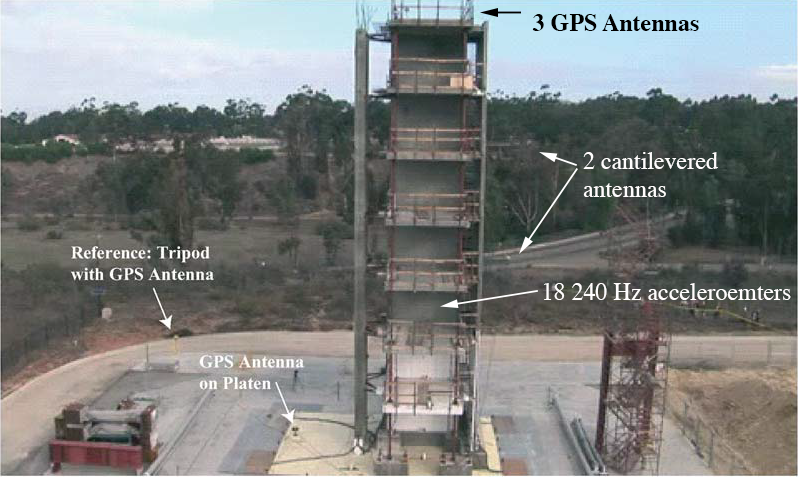
\includegraphics[width=0.99\linewidth]{./figures/ch2/shaketable2006.png}
    \caption[2006 shake table experiment configuration]{Experimental configuration for the 2006 shake table test}
  \label{fig_shake2006}
\end{figure}

The building was instrumented with seven geodetic-quality Navcom NCT-200D GPS receivers sampling at 50Hz and MEMS-Piezoresistive MSI model 3140 accelerometers sampling at 240Hz. Three GPS receivers were mounted on the roof (7th floor near the north, south and east corners), and two receivers were cantilevered on the 3rd and 5th floors of the flange wall (east side). A 6th receiver was located just off the shake table's platen as a stable reference poin for measuring displacements. A 7th GPS receiver was situated on the platen. The 15 accelerometers were mounted as follows: 2 on the platen, 4 on the building foundation, 3 on the first floor, 3 on the fifth floor and 3 on the seventh floor (roof). Unfortunately, the north receiver on the roof of the building was not operational during EQ4 due to a loose antenna cable. 

GPS phase and pseudorange data were streamed to a PC workstation and 50 Hz displacement waveforms were estimated on-the-fly using the method of instantaneous positioning (\citet{bock2000}) . The ``GPS-only'' displacements are relative to the fixed coordinates of the GPS receiver just off the platen, which were pre-determined with respect to the true-of-date ITRF2005 coordinates \citep{altamimi2007} of Plate Boundary Observatory (PBO) station P472 at Camp Elliot (32$^\circ$.8892N, 117$^\circ$.1047W), approximately 656 m away. The accelerometer data were doubly-integrated by high-pass filtering to determine ``accelerometer-only'' displacements. We re-sampled the 240Hz raw accelerometer data to 250Hz to be able to align the times of every 5th poin with the 50Hz Navcom GPS data. Displacement waveforms were then computed using both the forward and the smoothed Kalman (RTS) filter using the GPS platen data as input and, in turn, the raw data from the two platen and four foundation accelerometers. To assess accuracy, we compared the GPS-only, accelerometer-only, and Kalman filter displacements to the input ground truth displacements provided at 1024Hz by the MTS digital controller. To assess precision, we compared the root-mean-square (RMS) of the distances between pairs of accelerometers and pairs of GPS receivers on the roof of the building (7th floor). The results of these comparisons are given in Table \ref{tb_shakeresults}. 

\begin{longtable}{p{7cm} | p{1.4cm} | p{1.4cm} | p{1.4cm} | p{1.4cm}}
\caption[2006 shake table test results]{RMS differences between computed displacement waveforms and the input registered by the shake table's MTS recorder for four earthquake simulations (EQ1-EQ4). We show the results of high pass filtered accelerometer derived displacements for platen accelerometers (PA1 and PA2) and building foundation accelerometers (FA1-4) as well as Kalman filtered waveforms obtained from the platen GPS and platen and foundation accelerometers. We also show the results from decimated data (5 Hz for GPS and 100 Hz for accelerometers, and 1 Hz for GPS and 100Hz for accelerometers). The peak displacements are 0.16-0.17 m for EQ1-EQ3 and 0.40 m for EQ4} \label{tb_shakeresults}\\
\hline
\textbf{Sensors} & \textbf{EQ1} & \textbf{EQ2} & \textbf{EQ3} & \textbf{EQ4}\\
\hline
\multicolumn{5}{c}{\textbf{GPS Displacements RMS (m)}} \\
\hline
Platen GPS & 0.0026 & 0.0040 & 0.0029 & 0.0037\\
\hline
\multicolumn{5}{c}{\textbf{Accelerometer Derived Displacements RMS (m)}}\\
\hline
PA1 & 0.0193 & 0.0181 & 0.0151 & 0.0120\\
PA2 & 0.0177 & 0.0184 & 0.0131 & 0.0175\\
FA1 & 0.0308 & 0.0278 & 0.0037 & 0.0027\\
FA2 & 0.0304 & 0.0274 & 0.0036 & 0.0028\\
FA3 & 0.0307 & 0.0276 & 0.0037 & 0.0027\\
FA4 & 0.0307 & 0.0276 & 0.0036 & 0.0027\\
\hline
\multicolumn{5}{c}{\textbf{Forward Filter RMS (m)}}\\
\hline
PA1+GPS & 0.0021 & 0.0041 & 0.0034 & 0.0033\\
PA2+GPS & 0.0021 & 0.0041 & 0.0034 & 0.0033\\
FA1+GPS & 0.0016 & 0.0021 & 0.0020 & 0.0020\\
FA2+GPS & 0.0016 & 0.0020 & 0.0020 & 0.0020\\
FA3+GPS & 0.0016 & 0.0021 & 0.0020 & 0.0020\\
FA4+GPS & 0.0016 & 0.0021 & 0.0020 & 0.0020\\
\hline
\multicolumn{5}{c}{\textbf{Forward Filter + 5 Hz Decimation RMS (m)}}\\
\hline 
PA1+GPS & 0.0041 & 0.0074 & 0.0074 & 0.0046\\
PA2+GPS & 0.0040 & 0.0074 & 0.0074 & 0.0046\\
FA1+GPS & 0.0042 & 0.0067 & 0.0063 & 0.0037\\
FA2+GPS & 0.0042 & 0.0066 & 0.0063 & 0.0037\\
FA3+GPS & 0.0042 & 0.0066 & 0.0063 & 0.0037\\
FA4+GPS & 0.0042 & 0.0066 & 0.0063 & 0.0037\\
\hline
\multicolumn{5}{c}{\textbf{Forward Filter + 1 Hz Decimation RMS (m)}}\\
\hline
PA1+GPS & 0.0353 & 0.0211 & 0.0625 & 0.0341\\
PA2+GPS & 0.0353 & 0.0211 & 0.0625 & 0.0341\\
FA1+GPS & 0.0333 & 0.0313 & 0.0612 & 0.0273\\
FA2+GPS & 0.0333 & 0.0305 & 0.0607 & 0.0265\\
FA3+GPS & 0.0333 & 0.0308 & 0.0609 & 0.0275\\
FA4+GPS & 0.0333 & 0.0309 & 0.0601 & 0.0277\\
\hline
\multicolumn{5}{c}{\textbf{Forward Filter + RTS Smoothing RMS (m)}}\\
\hline
PA1+GPS & 0.0016 & 0.0036 & 0.0024 & 0.0028\\
PA2+GPS & 0.0016 & 0.0036 & 0.0024 & 0.0028\\
FA1+GPS & 0.0017 & 0.0021 & 0.0021 & 0.0025\\
FA2+GPS & 0.0017 & 0.0021 & 0.0021 & 0.0025\\
FA3+GPS & 0.0017 & 0.0021 & 0.0021 & 0.0025\\
FA4+GPS & 0.0017 & 0.0021 & 0.0021 & 0.0025\\
\hline
\multicolumn{5}{c}{\textbf{Forward Filter + RTS Smoothing + 5 Hz Decimation RMS (m)}}\\
\hline
PA1+GPS & 0.0015 & 0.0038 & 0.0027 & 0.0028\\
PA2+GPS & 0.0015 & 0.0038 & 0.0027 & 0.0028\\
FA1+GPS & 0.0017 & 0.0022 & 0.0024 & 0.0025\\
FA2+GPS & 0.0017 & 0.0022 & 0.0024 & 0.0025\\
FA3+GPS & 0.0017 & 0.0022 & 0.0024 & 0.0025\\
FA4+GPS & 0.0017 & 0.0022 & 0.0024 & 0.0025\\
\hline
\multicolumn{5}{c}{\textbf{Forward Filter + RTS Smoothing + 1 Hz Decimation RMS (m)}}\\
\hline
PA1+GPS & 0.0077 & 0.0102 & 0.0152 & 0.0130\\
PA2+GPS & 0.0077 & 0.0102 & 0.0152 & 0.0130\\
FA1+GPS & 0.0097 & 0.0117 & 0.0168 & 0.0115\\
FA2+GPS & 0.0097 & 0.0118 & 0.0166 & 0.0115\\
FA3+GPS & 0.0098 & 0.0117 & 0.0167 & 0.0114\\
FA4+GPS & 0.0096 & 0.0117 & 0.0167 & 0.0115\\
\hline
\multicolumn{5}{c}{\textbf{Roof Baselines RMS (m)}}\\
\hline
GPS (N-S) & 0.0033 & 0.0026 & 0.0035 & n/a\\
GPS (N-E) & 0.003 & 0.0019 & 0.0034 & n/a\\
GPS (S-E) & 0.0036 & 0.0033 & 0.0023 & 0.0031\\
Accelerometer (N-S) & 0.0008 & 0.0007 & 0.001 & 0.0012\\
\hline
\end{longtable}

\subsubsection{Accuracy of the Displacement Waveforms}

Accuracy was determined by comparing the various displacement waveforms with the``true'' displacements provided by the MTS recorder, for each of the four experiments, using the RMS difference as the statistical measure. The results are given in Figure \ref{fig_shakewaves} and Table \ref{tb_shakeresults}. The peak-to-peak displacements are on the order of 0.17 m for EQ1-EQ3, and 0.4 m for the high intensity Northridge event (EQ4). The RMS statistic is computed over the entire record including dynamic and static periods. The displacements for the single GPS on the platen have an RMS difference of 2.6-4.0mm, while the displacements for the two accelerometers on the platen have an RMS difference of 12.0-19.3mm. The larger differences for the accelerometer-derived displacements result from mismatches in amplitude and phase compared to the MTS displacements. The forward Kalman filter solutions reduce the RMS differences by about 10\% (except for EQ2 where there is a 10\% increase) compared to the GPS-only solutions (2.2-4.1mm), and there is an additional 10\% improvement for all four experiments with the smoothed Kalman filter solutions (1.6-2.3mm). For the foundation accelerometers, the RMS differences are higher for EQ1 and EQ2 (about 30mm), but unexpectedly an order of magnitude less for EQ3 and EQ4. In any case, we can conclude that the combined GPS and accelerometer displacement waveforms provide overall mm-level accuracy over the entire range of sampled frequencies, and improved accuracy when compared to GPS-only or accelerometer-only solutions. The improvement is generally more pronounced when compared to the accelerometer-only solutions. This is not surprising because of the inherent limitations and biases encountered in the double integration of accelerometer data.  It is interesting to note that the RMS statistics for either the static or dynamic periods did not differ significantly from the RMS values computed for the entire period (static and dynamic) for any of the experiments. We saw only insignificant degradation (10\%) in accuracy during periods of strong shaking.

\begin{figure}[!ht] 
\centering
  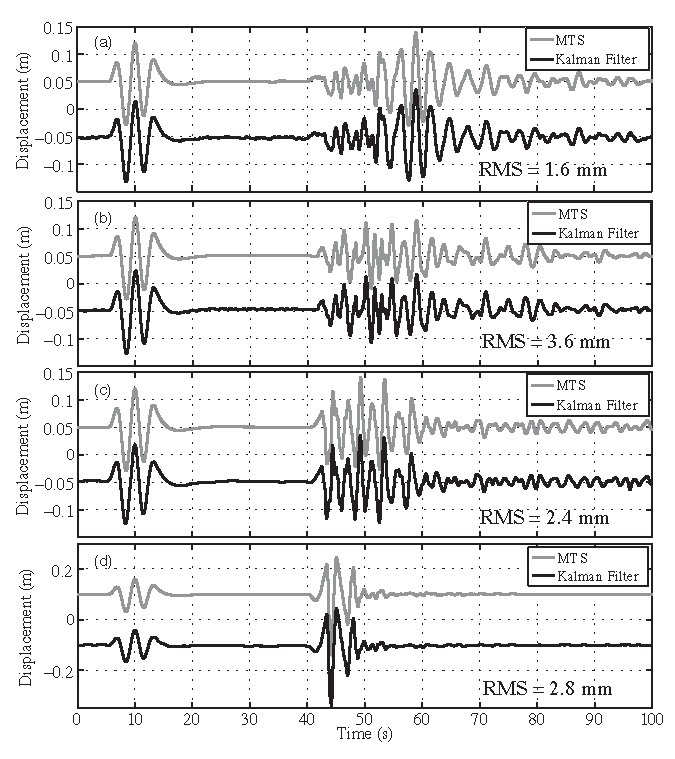
\includegraphics[width=0.99\linewidth]{./figures/ch2/shake_waves.pdf}
    \caption[2006 shake table experiment Kalman filtered waveforms]{Accuracy of broadband displacement waveforms. Root-mean-square (RMS) of the differences between the smoothed Kalman filter displacement waveforms estimated for the four earthquake simulations and the deterministic input as registered at 1024 Hz by the shake table's MTS digital recorder (see also Table \ref{tb_shakeresults}). The waveforms are estimated from the platen GPS and one of the accelerometers on the platen. Note that the vertical scale is the same for (a) through (c) but changes for (d). The two waveforms in each graph have been offset for clarity.}
  \label{fig_shakewaves}
\end{figure}

We repeated the previous analysis with two decimation schemes: the first one decimating the accelerometer to 100Hz and the GPS to 5Hz and the second one decimating the accelerometer to 100Hz and the GPS to 1Hz (Table \ref{tb_shakeresults}). The latter corresponds to the sampling rates of real-time GPS and strong motion sensors in southern California during the 2010 $M_w$7.2 El Mayor-Cucapah earthquake. We find that the fit of the Kalman filtered waveforms is only mildly degraded in the first decimation scheme, and significantly degraded with the second decimation scheme. However smoothing provides a significant improvement, especially at the lower GPS sampling rates (1Hz). This is an important practical consideration since GPS data are considerably more verbose than strong motion data. 

\subsubsection{Precision of the Displacement Waveforms}

In order to evaluate precision we examined the RMS of the difference in displacements estimated for pairs of GPS and pairs of accelerometers on the roof of the building (7th floor) for each of the four experiments (Figure \ref{tb_shakeresults}), including periods of both quiet and dynamic motion. The assumption is that the roof is rigid, and that there is no permanent deformation occurring between the sensors. The displacements obtained from high pass filtering of the accelerometer data show smaller RMS differences on the order of only 1mm while the GPS-only displacements show RMS differences on the order of 3mm. This makes sense since accelerometer data are more sensitive to ground motion than GPS data, that is, they are more precise. However, as we have seen accuracy is degraded for the accelerometer displacements due to biases in the double integration process, which in this case appear to be common to both accelerometers on the roof. GPS precision of about 3mm is what we would expect from earlier studies of high-rate GPS horizontal displacements on short baselines \citep{genrich2006}.

\subsection{The 2010 $M_w$7.2 El Mayor-Cucapah Earthquake}

The shake table experiments differed from a real-world event in several important ways. First, only the dynamic motions could be simulated. In a real event there would be no nearby stable GPS reference station and displacements would need to be referred to one or more stations outside the region of deformation. Also, GPS noise would increase with longer station separations, by a factor of about 3 in the horizontal components and up to an order of magnitude in the vertical component \citep{langbein2004,genrich2006}. Finally, the ability to resolve integer-cycle phase ambiguities in real-time scenarios is diminished as station separations increase \citep{bock2000}. The 2010 $M_w$7.2 El Mayor-Cucapah earthquake in northern Baja California and observations from southern California high-rate GPS and very-high-rate accelerometers provide us with a real-world event to highlight the advantages of combining GPS displacements and acceleration data.

The El Mayor-Cucapah earthquake broke a subset of northwest-trending strike-slip faults that are separated by pull-apart basins that accommodate northwest-southeast oriented extension, and are parallel to the main strands of the San Andreas fault system (Imperial, Elsinore, San Jacinto, Laguna Salada, and Cerro Prieto faults). It caused significant ground motions at distances up to several hundred kilometers from the epicenter \citep{hauksson2011,wei2011}. A robust set of 1Hz GPS phase and pseudorange data were collected for this earthquake at 105 California Real-Time Network (CRTN) and PBO stations (Figure \ref{fig_mapelmayor}) and on-the-fly displacement waveforms were estimated.

\begin{figure}[!ht] 
\centering
  \includegraphics[width=0.99\linewidth]{./figures/ch2/map_elmayor.pdf}
    \caption[Station distribution for the El Mayor Cucapah earthquake]{California Real Time GPS Network (CRTN) stations in southern California and collocated California Integrated Seismic Network (CISN) strong-motion accelerometer stations. The arrows indicate horizontal coseismic offsets from the 2010 $M_w$7.2 El Mayor-Cucapah earthquake. The 12 collocated stations (where the GPS and strong-motion accelerometers are within 1.5 km) are denoted by white diamonds. The GPS station name is given by its 4-character code, and the seismic station by its 3-character code. P494/WES has a broadband seismometer, an accelerometer, and a GPS receiver and is featured in several subsequent figures.}
  \label{fig_mapelmayor}
\end{figure}
 
In order to evaluate the Kalman filter performance, we reprocessed the entire set of 1 Hz GPS-derived displacement waveforms (Figure \ref{fig_elmay_allwaves}) in simulated real-time mode using the network approach. We divided the network into 9 subnetworks with at least 2-station overlap and estimated relative displacement waveforms in the ITRF2005 frame for each subnetwork relative to an arbitrary station within each. The maximum relative motion encountered between adjacent stations closest to the epicenter was 0.58 m between stations P494 and P497 located 16.7km apart (Figure \ref{fig_mapelmayor}). Then, we performed a network adjustment to estimate coordinates for all stations with respect to the true-of-date coordinates of station GNPS, and transformed the coordinates for each station into displacements in the local (N,E,U) frame using Equation \ref{eq_rot}. GNPS was chosen not because it is the farthest from the epicenter (it is 245 km to the northeast, Figure \ref{fig_mapelmayor}), but because of directivity considerations. 

\begin{figure}[!ht] 
\centering
  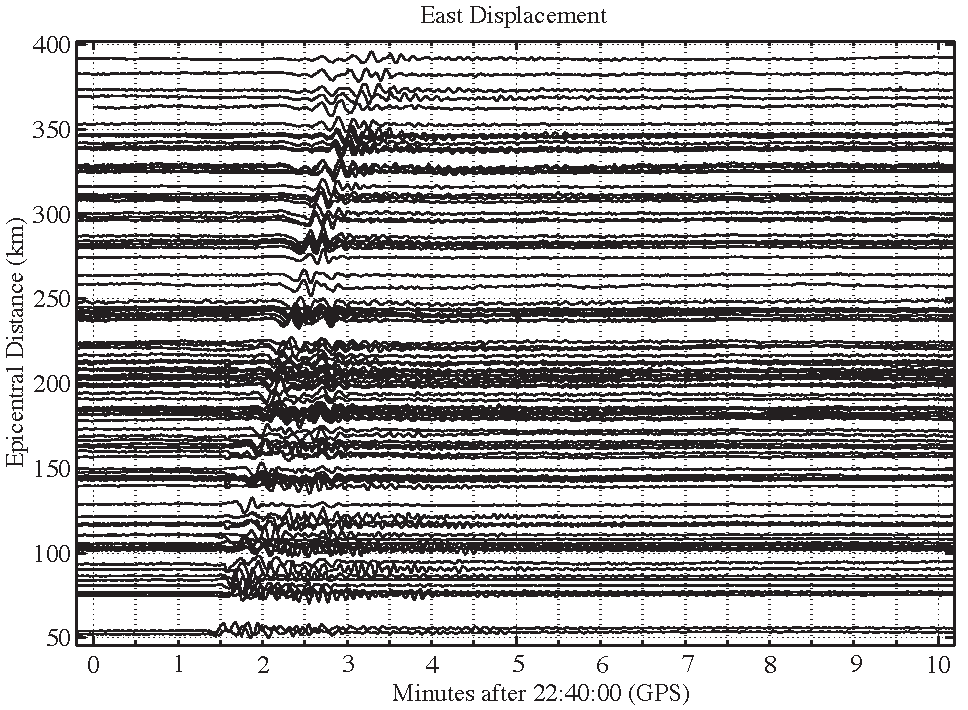
\includegraphics[width=0.99\linewidth]{./figures/ch2/elmay_allwaves.pdf}
    \caption[GPS waveforms for the El Mayor Cucapah earthquake]{1 Hz (East component) displacements estimated for 105 CRTN stations are plotted according to epicentral distance for the April 4, 2010 $M_w$7.2 El Mayor-Cucapah earthquake. The earthquake initiated at 22:40:40 UTC, or equivalently 22:40:55 GPS time. All waveforms have been normalized for clarity}
  \label{fig_elmay_allwaves}
\end{figure}

We then combined the GPS-derived 1Hz displacements with raw 100Hz accelerometer data using the Kalman forward and smoothed filters to estimate the velocity and displacement waveforms. This was performed on a station-by-station basis for those 12 GPS stations that were within 1.5km of an accelerometer. The instruments closest to the earthquake's epicenter were the accelerometer at WES and GPS at P494 (Table \ref{tb_elmay_sta}). The two sensors are about 72km from the epicenter just north of the U.S.-Mexico border and 80m from each other (Figure \ref{fig_mapelmayor}). 

\begin{table}
\caption[Collocated GPS and strong-motion stations in Southern California]{Collocated GPS (California Real Time GPS Network) and strong-motion accelerometer (California Integrated Seismic Network) stations with a station separation of 1.5 km or less.}
\label{tb_elmay_sta}
\begin{tabular}{l | c | c | l | c | c | c}
\hline
CRTN&Latitude&Longitude&SCSN&Latitude&Longitude&Separation\\
Station&$^\circ$N&$^\circ$W&Station&$^\circ$N&$^\circ$W&km\\
\hline
P473 & 32.7338 & 116.9495 & SDR & 32.7356 & 116.9424 & 0.7\\
P494 & 32.7597 & 115.7321 & WES & 32.7590 & 115.7316 & 0.08\\
GMPK & 33.0511 & 114.8273 & GLA & 33.0512 & 114.8271 & 0.05\\
SLMS & 33.2922 & 115.9778 & SAL & 33.2801 & 115.9859 & 1.50\\
PMOB & 33.3572 & 116.8595 & PLM & 33.3536 & 116.8626 & 0.5\\
BOMG & 33.3646 & 115.7297 & BOM & 33.3647 & 115.7296 & 0.01\\
SBCC & 33.5530 & 117.6615 & SDD & 33.5526 & 117.6617 & 0.05\\
THMG & 33.6506 & 116.0773 & THM & 33.6507 & 116.0773 & 0.01\\
CACT & 33.6551 & 115.9900 & CTC & 33.6551 & 115.9901 & 0.01\\
VTIS & 33.7126 & 118.2938 & FMP & 33.7126 & 118.2938 & 0.00\\
SNOG & 34.0352 & 116.8078 & SNO & 34.0352 & 116.8078 & 0.01\\
MSCG & 34.0385 & 116.6480 & MSC & 34.0385 & 116.648 & 0.00\\
\hline
\end{tabular}
\end{table}

In Figure \ref{fig_wes_p494_all}a, we show the entire period of seismic shaking at P494/WES in the vertical component. The observed broadband velocities clip before the arrival of the \textit{S} wave at the station, while the estimated velocity waveforms record the entire event at the 100Hz rate of the accelerometer. In Figure \ref{fig_wes_p494_all}b, we show the first 12s of the vertical broadband seismometer record at WES after the Southern California Earthquake Center's \textit{P} wave pick and overlay the Kalman-filter-estimated velocities. That the broadband seismic data and the waveform estimated by Kalman smoothing are indistinguishable is striking, given also that the GPS resolution is poorest in the vertical direction. In Figure \ref{fig_wes_p494_all}c, we compare displacements derived by (single) integration of the (12s) seismometer record at WES, and the 100Hz smoothed Kalman filter broadband displacements. it is clear that we can detect the small-amplitude \textit{P} wave recordings with a precision (and accuracy) of about 1mm. This is a significant improvement over the 1Hz GPS-only solutions where the vertical precision is on the order of several tens of millimeters, often precluding \textit{P} wave detection.

\begin{figure}[!ht] 
\centering
  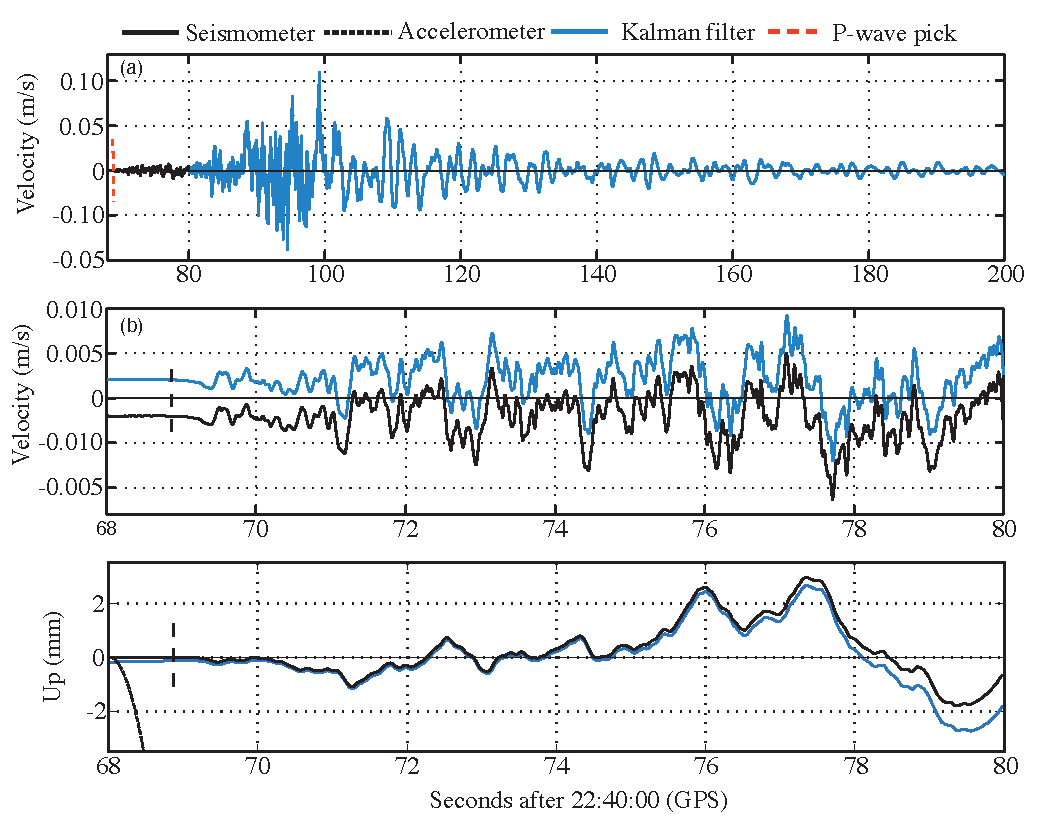
\includegraphics[width=0.99\linewidth]{./figures/ch2/wes_p494_all.pdf}
    \caption[Kalman filtered waveforms for WES/P494]{Estimation of velocity and displacement waveforms. (a) Comparison between vertical velocity records registered by a broadband seismometer at station WES (Figure \ref{fig_mapelmayor}) which clipped 11 seconds after the onset of shaking and the smoothed Kalman filter estimated velocities for P494/WES. (b) Blowup of the same time series showing agreement between the observed velocity and the estimated Kalman velocity waveforms. The two waveforms have been offset for clarity. The SCEC \textit{P} wave pick denoted by vertical dashes is at ~22:41:09 GPS time, or 29 seconds after earthquake initiation. (c) Comparison of single integration of the vertical seismometer record at WES, 100 Hz smoothed Kalman filter displacements (GPS/accelerometer), and double integration of only the accelerometer data. Note the magnitude of displacement, indicating that the broadband displacements have a precision and accuracy of about 1 mm.}
  \label{fig_wes_p494_all}
\end{figure}


Figure \ref{fig_wes_p494_all}c also shows the poor results obtained by on-the-fly double integration of the accelerometer data. Of course, better results could be obtained after the fact with post-processed baseline corrections. To investigate this we computed displacements for WES from uncorrected double integration of accelerometer data (0-th order correction), correcting with the BI baseline removal scheme (Section \ref{sec:strongmotion}), and with high pass filtering. Although the dynamic motions could be extracted through baseline corrections or function fitting, the static displacements were lost. With the addition of high-rate GPS displacements, high pass filtering or function fitting is not required, and the double integration can be performed on-the-fly using just the raw accelerometer records. In Section \ref{sec:tohoku} we will quantify the performance of baseline correction schemes when compared to the Kalman filter when we consider the Tohoku-oki data.

In Figure \ref{fig_weskal}, we show the broadband displacement waveforms for P494/WES in all 3 components, where the 0.2m horizontal static offset in the North component is clearly seen. The corresponding smoothed Kalman filter vertical displacement waveforms for P494/WES, as well as those for two other collocated GPS/accelerometer stations (BOMG/BOM and THMG/TGM, 129 and 192 km from the epicenter, respectively; Figure \ref{fig_mapelmayor} and Table \ref{tb_elmay_sta}) are shown in Figure \ref{fig_kal_3verts}. In spite of the larger epicentral distance and the diminished precision of the GPS vertical component, the Kalman filter with the aid of the accelerometer data is still capable of producing a precise waveform.

\begin{figure}[!ht] 
\centering
  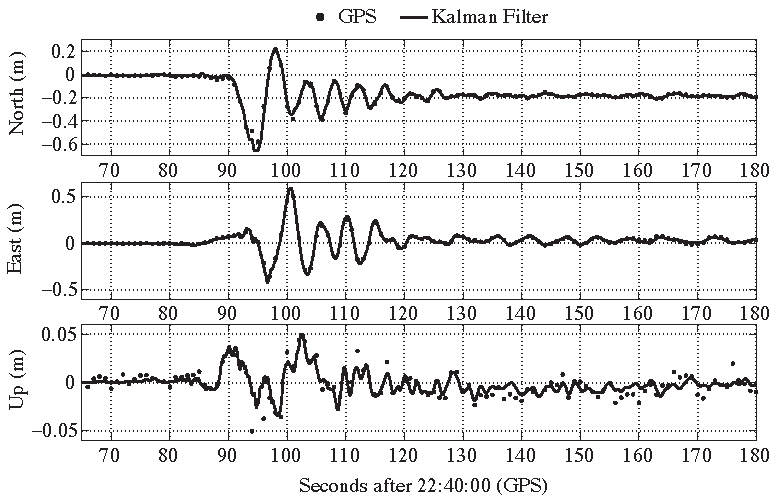
\includegraphics[width=0.99\linewidth]{./figures/ch2/weskal.pdf}
    \caption[GPS and Kalman filtered displacements at P494/WES]{Comparison of 1Hz GPS and 100Hz smoothed Kalman filter displacement waveforms. Shown are 1Hz GPS displacements for P494 and 100Hz smoothed Kalman filter displacements for P494/WES. The SCEC \textit{P} wave pick for station WES is at ~22:41:09 GPS time. Note the 0.2m static (coseismic) offset in the North component}
  \label{fig_weskal}
\end{figure}

\begin{figure}[!ht] 
\centering
  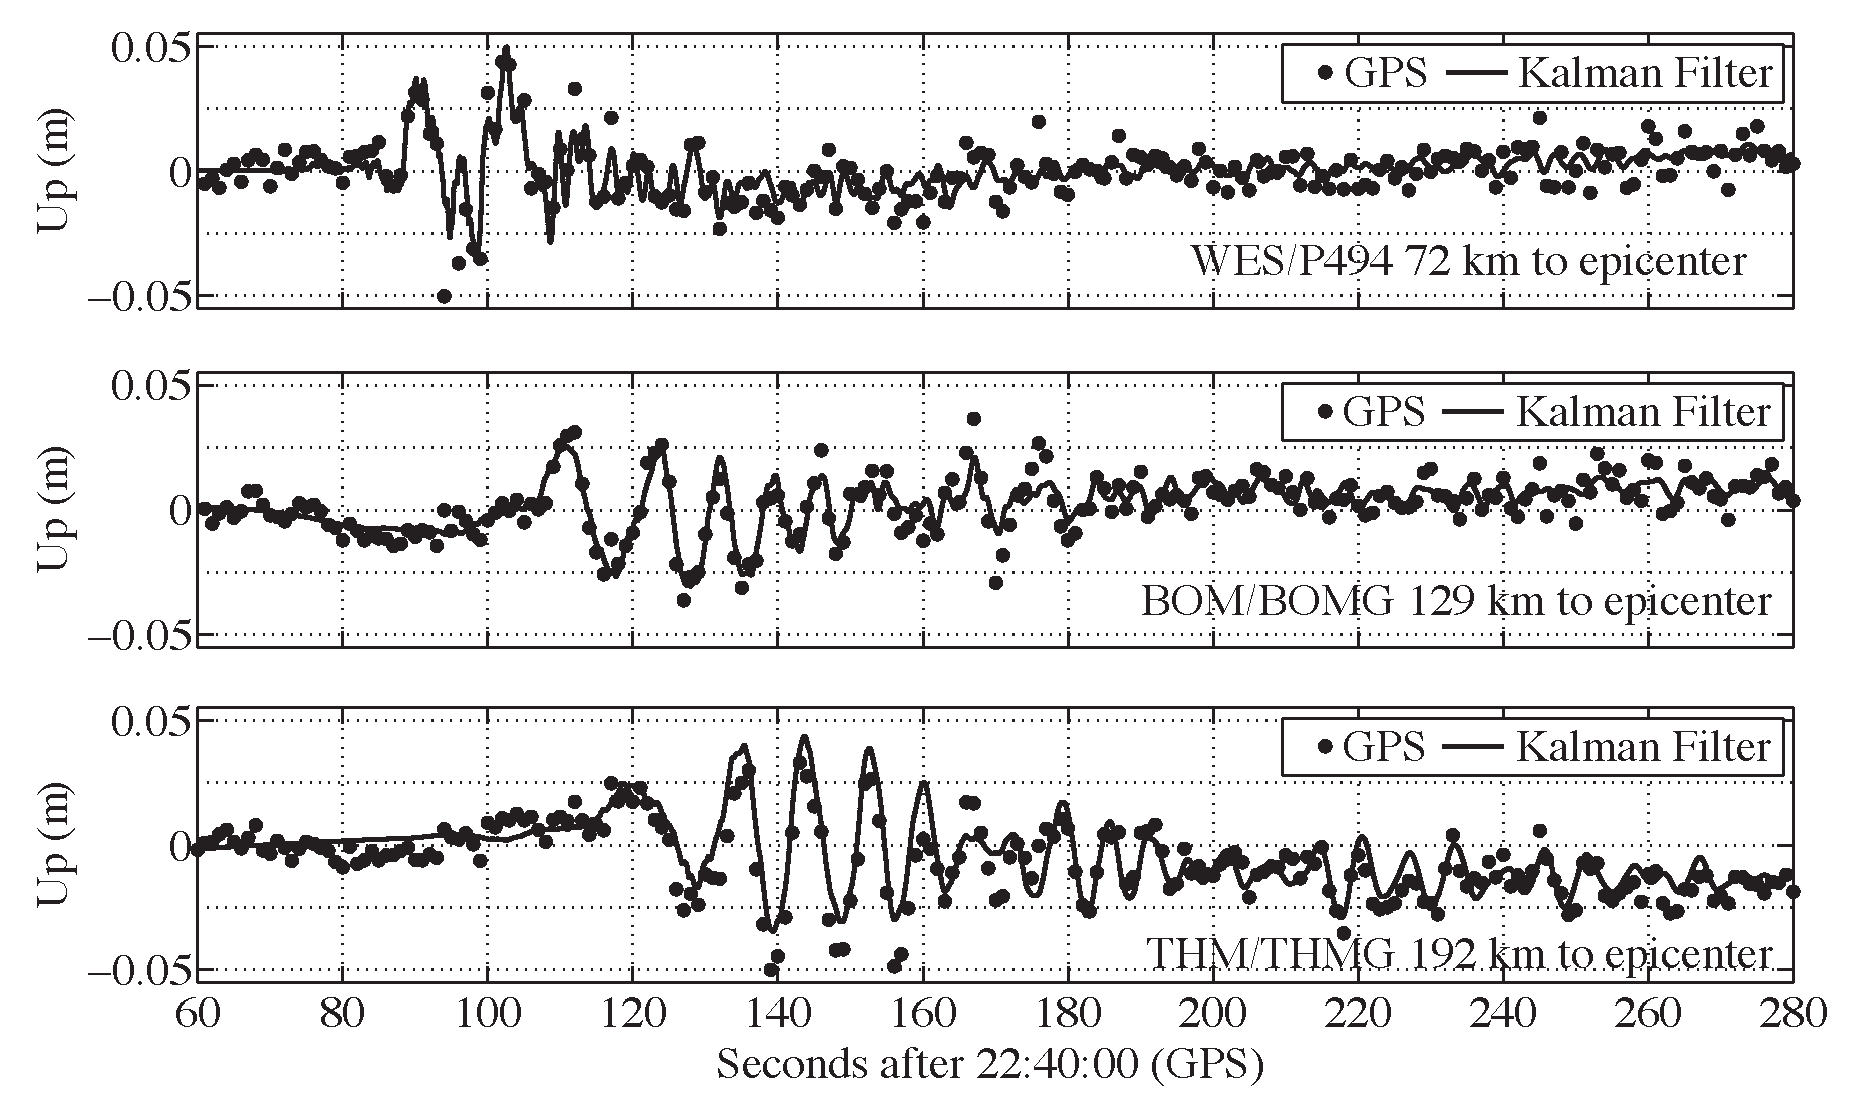
\includegraphics[width=0.99\linewidth]{./figures/ch2/kal_3verticals.pdf}
    \caption[Vertical Kalman filter performance]{ Vertical displacement waveforms. Comparison of 1Hz GPS and 100Hz smoothed Kalman filter estimates for P494 and P494/WES, BOMG and BOMG/BOM, and THMG and THMG/THM.}
  \label{fig_kal_3verts}
\end{figure}

\subsection{Spectral Characteristics}
Spectral analysis of the smoothed Kalman filter displacement time series for the shake table experiments (Figure \ref{fig_elmay_shake_psd}a) and the El Mayor-Cucapah earthquake (Figure \ref{fig_elmay_shake_psd}b) highlights two attractive features: the power spectral densities follow the GPS-only spectrum at the low frequencies and the accelerometer-only spectrum at the high frequencies. This is desirable because it is in these two frequency bands that each instrument performs best (GPS at the lower frequencies and accelerometers at the higher frequencies). We can infer from the power spectral densities and the shake table experiments that the combined (100 Hz) waveform is more precise and accurate than the (1Hz) GPS-only or (100Hz) accelerometer-only displacement waveforms, and that we have achieved an accurate broadband record of this event.

\begin{figure}[!ht] 
\centering
  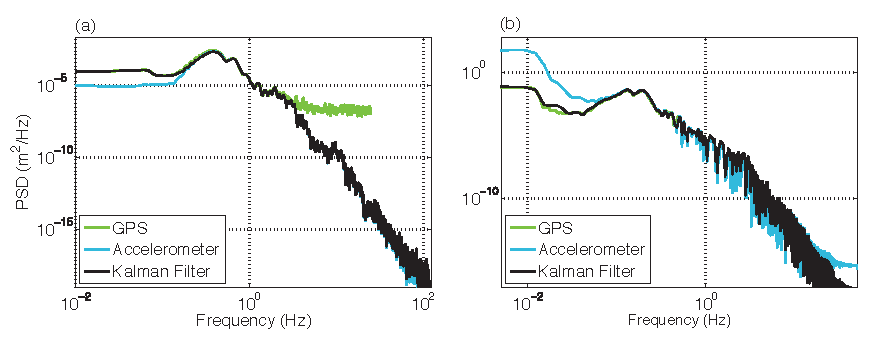
\includegraphics[width=0.99\linewidth]{./figures/ch2/elmay_shake_psd.pdf}
    \caption[Shaketable and El Mayor-Cucapah Kalman filter PSDs]{Power spectral densities. (a) High intensity Northridge earthquake simulation (EQ4) on shake table platen for 50Hz GPS-only displacements, 240Hz accelerometer-derived high-pass filtered displacements, and 250Hz smoothed Kalman filter displacements; (b) 2010 El Mayor-Cucapah earthquake for 1Hz GPS displacements at P494, 100Hz accelerometer-derived high-pass filtered displacements at WES, and 100Hz smoothed Kalman filter displacements for P494/WES.}
  \label{fig_elmay_shake_psd}
\end{figure}

The smoothed Kalman filter cannot be performed in real time since it requires both a forward and backward step. However, an examination of the spectral characteristics of the forward filter displacements indicates spurious spectral peaks that coincide with multiples of the GPS sampling frequency for both the shake table experiments (Figure \ref{fig_psd_peaks}a) and the El Mayor-Cucapah earthquake (Figure \ref{fig_psd_peaks}). it is easy to see why this happens by examination of a blowup of 1s of the unsmoothed forward time series for the shake table experiment (Figure \ref{fig_kal_saw}). In between the 50Hz GPS samples, the series drifts during successive time updates when only new accelerometer data are available (every 250th of a second for the shake table and every 100th of a second for the earthquake).  But as soon as the next GPS measurement becomes available there is an adjustment to the displacement time series, explaining the observed saw tooth pattern, a pattern also evident in the El Mayor-Cucapah earthquake data. In Figure \ref{fig_synth_saw}, we show the results of a synthetic test of a saw tooth with a period of 1s and estimate its power spectral density using the multitaper method. It shows broad peaks centered at multiples of the saw tooth period, which corresponds to the GPS sampling frequency in our data sets. This is a minor problem because for real-time seismological applications the increase in noise introduced by the peaks is small compared to the signal. Furthermore, the increase in noise is only at frequencies higher than ~1-2 Hz. In any case, the fixed interval smoother removes the spurious peaks altogether, while the near-real-time smoother will reduce the noise peaks as a function of the smoother lag time.

\begin{figure}[!ht] 
\centering
  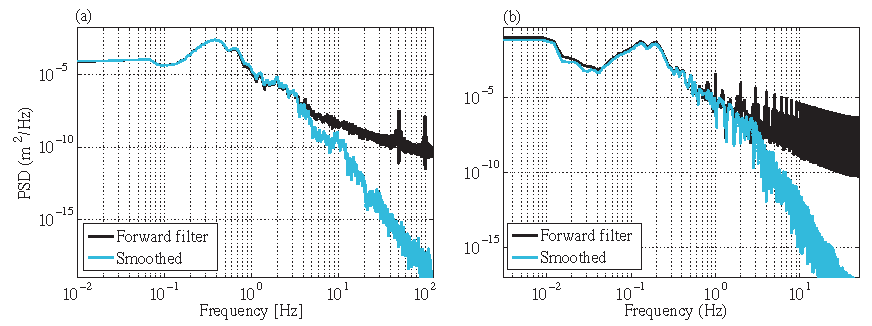
\includegraphics[width=0.99\linewidth]{./figures/ch2/psd_peaks.pdf}
    \caption[Comparisson of forward and smoothed Kalman filter PSDs]{Power spectral density comparisons between forward Kalman filter and smoothed Kalman filter displacements waveforms for (a) High intensity Northridge earthquake simulation (EQ4) 250 Hz displacements on shake table platen; (b) 2010 El Mayor-Cucapah earthquake 100Hz displacements for P494/WES. Note the spikes in the forward filter corresponding to the GPS sampling frequency, 50Hz for (a) and 1Hz for (b).}
  \label{fig_psd_peaks}
\end{figure}

\begin{figure}[!ht] 
\centering
  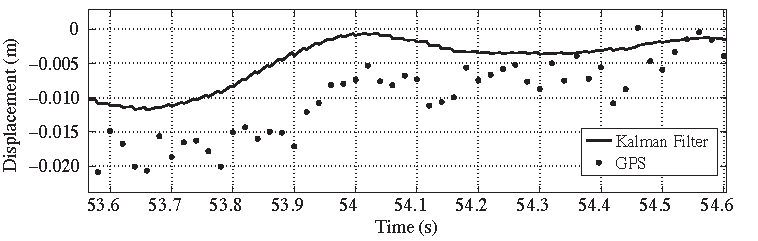
\includegraphics[width=0.99\linewidth]{./figures/ch2/kal_saw.pdf}
    \caption[Forward filter sawtooth effects]{Example of saw-tooth like irregularities introduced by the disparity in sensor sampling frequencies. Shown is a blowup of the high intensity Northridge earthquake simulation (EQ4) with a 250Hz sampling frequency for the forward Kalman filter displacements and 50Hz sampling frequency for the GPS-only displacements.}
  \label{fig_kal_saw}
\end{figure}

\begin{figure}[!ht] 
\centering
  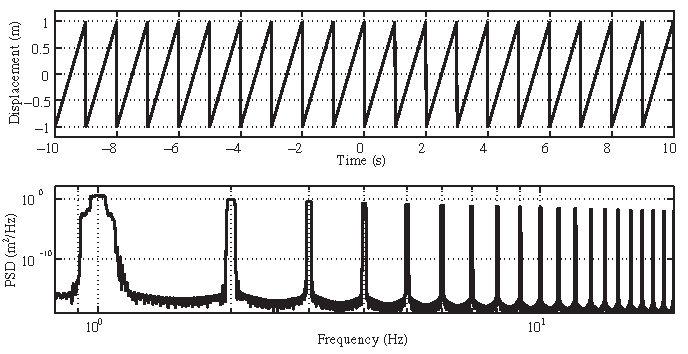
\includegraphics[width=0.99\linewidth]{./figures/ch2/synth_saw_psd.pdf}
    \caption{1Hz synthetic saw tooth and its power spectral density.}
  \label{fig_synth_saw}
\end{figure}

\subsection{Selecting the Kalman Filter Variances}

The Kalman filter has two parameters that dictate its performance, the measurement variance $r$ and the system dynamics variance $q$ (Section \ref{Section sec:kalman}). To maintain objectivity and to simulate a real-time environment we compute the measurement variance from 50s windows of pre-event noise on the 3 components of the GPS displacements (Figure \ref{fig_variances}). These tend to be very stable across a network with the East component showing the least variance, then the North component and the vertical component being the noisiest, as expected, due to the satellite constellation configuration and unmodeled tropospheric refraction \citep{bock2000}. The observed GPS variances are also consistent with the results of \citet{genrich2006} who analyzed high-rate real-time data in Southern California.

\begin{figure}[!ht] 
\centering
  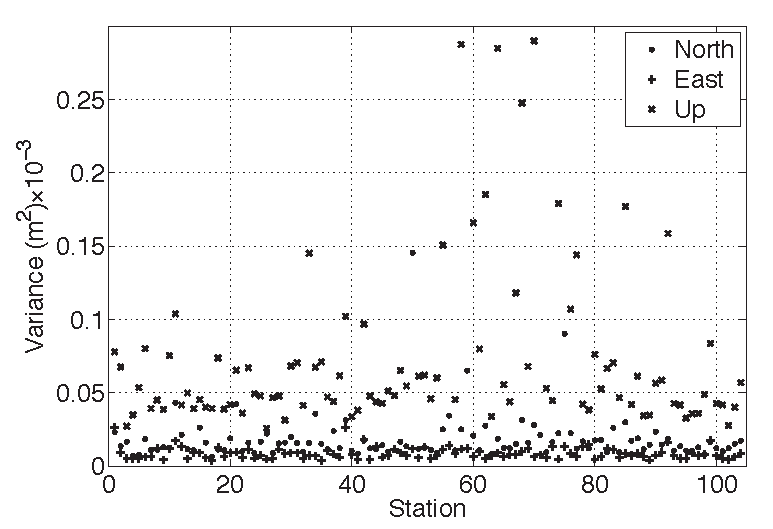
\includegraphics[width=0.99\linewidth]{./figures/ch2/variances.pdf}
    \caption[Noise variances at CRTN GPS stations]{Variances for 50 seconds of displacements for some California Real Time GPS Network (CRTN) stations estimated prior to the 2010 El Mayor-Cucapah earthquake in North, East, and Up components.}
  \label{fig_variances}
\end{figure}

Estimating the system dynamics variance is more complicated. At first glance it could be determined simply by taking the variance of windows of pre-event accelerometer noise. However, there are several sources of noise in the accelerometer that preclude this. Perhaps the most important is sensor rotation and tilt \citep{Trifunac2001,Pillet2007} whose net effect is to raise the noise floor. This does not manifest itself until shaking starts and is thus not present in pre-event noise estimation. \citet{Trifunac2001} show that as one utilizes an increasing number of bits to digitize the transducer signal and as earthquake magnitude increases the problem becomes more insidious. \citet{lee2009} obtained empirical relations for computing the Fourier spectra of rotation and tilt from translational acceleration spectra. The empirical relations depend on multiple factors including magnitude, focal depth, soil conditions, thickness of the sedimentary layer and epicentral distance. When compared to the amplitudes of processing and recording noise however, they find that the most extreme behavior of the rotational and tilting spectra is about 3 orders of magnitude greater than translational noise levels. We show the effect of using $q$ measured from pre-event noise windows by taking the more extreme value of $1000q$ as the system dynamics variance for input into the Kalman filter. In Figure \ref{fig_qeffect}a we show the East component (because it displays the largest sensitivity to changes in $q$) and observe that when applying the forward Kalman filter without smoothing and comparing it to GPS measurements the filter miscomputes the resulting static displacements by as much as 0.08m. If we adjust the variance to $1000q$ then the static offset is adequately recovered but the amplitudes of dynamic shaking can vary by as much as 0.25m.

\begin{figure}[!ht] 
\centering
  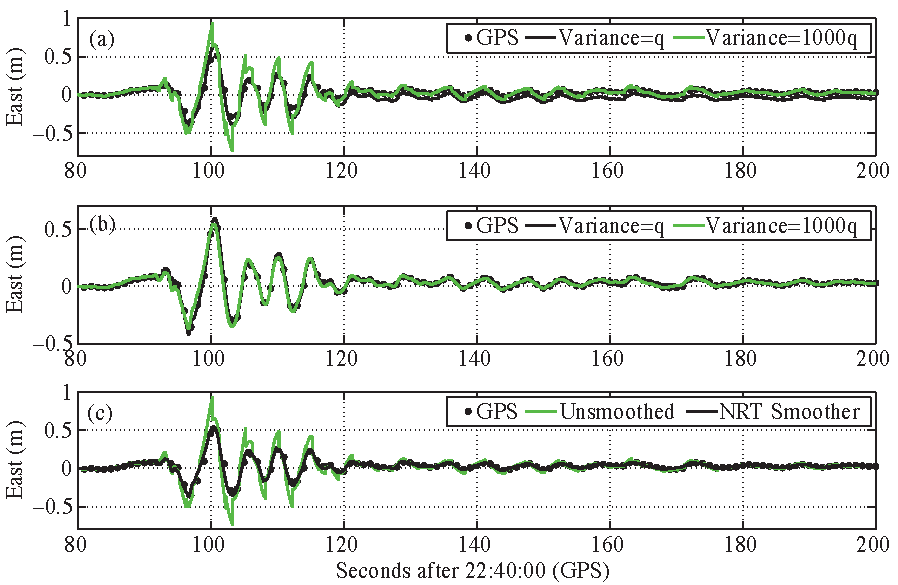
\includegraphics[width=0.99\linewidth]{./figures/ch2/qeffect.pdf}
    \caption[Sytem dynamics variance and its effect on the Kalman filter]{Effect of choice of system dynamics variance in Kalman filter estimation, in the East component. (a) Comparison between forward Kalman filter waveforms using $q$ and $1000q$ as the system dynamics variance, where q is the pre-event variance estimate for the accelerometer data. (b) Comparison between RTS smoothed waveforms using $q$ and $1000q$ as system dynamics variance. (c) Comparison between forward Kalman filter and smoothed Kalman filter with a lag of 10s using $1000q$. }
  \label{fig_qeffect}
\end{figure}

In spite of these large variations, the problem becomes, in effect, moot using Kalman smoothing, where using a scaled value of $q$ has a limited effect on the recovered waveform (Figure \ref{fig_qeffect}b). Applying a near-real-time smoother (Section \ref{sec:kalman}) with a 10s lag, even with an extreme value of the variance, fully recovers the waveform (Figure \ref{fig_qeffect}c). We find that the 10 s lag, in this case, is the minimum necessary to recover an adequate waveform, that is, one without bias in dynamic shaking amplitude or in static offset. This lag, however, might be too long for real-time applications in which case the sampling rate of the GPS must be increased to reduce the lag of the near-real-time smoother (recall that misfits arise from the saw tooth pattern effect of GPS sampling frequency). Alternatively, if the station conditions are known, the empirical relations of \citet{lee2009} or some yet to be determined empirical scheme can be used to assess the proper scaling of $q$.

\subsection{Lessons and Insights}

As a proof of concept, the shake table tests and the recordings of the El Mayor-Cucuapah earthquake allowed us to better understand the operational characteristics of the Kalman filtering operation.

The very-high frequency response of GPS-derived displacements is flat above 0.05-0.5Hz ($<$2-20 s) so that GPS data are capable of providing essentially uncorrelated single-epoch estimates of displacement over a large range of frequencies at the (10-50Hz) sampling rate of modern GPS receivers \citep{genrich2006}. The California Real-Time Network project (http://sopac.ucsd.edu/projects/realtime) has demonstrated that 10Hz data can be reliably streamed over dedicated microwave and radio modem communication links but this requires a ten-fold increase in the transmitted data compared to the current 1Hz rate. The Plate Boundary Observatory project (http://pbo.unavco.org) streams 1Hz data from their GPS stations but stores 10Hz measurements in receiver memory which can be downloaded in the case of a significant seismic event. It is not practical to stream at higher data rates with current costs and limitations in telemetry. A more cost-effective approach is to, wherever possible, add accelerometer instruments at existing GPS stations, stream the very-high-rate but lower volume accelerometer data over the same communications links as the GPS data, and use the Kalman filter to optimally combine both data sets. One might even consider performing the filtering operation which is computationally simple at the station itself. This approach provides displacements at the sampling rate of the accelerometers (e.g., 100Hz) with the precision of the accelerometer data and the accuracy of the GPS data. Our shake table results indicate that there is little benefit in increasing the GPS sampling rate to greater than 5-10Hz.
 
We find that the basic state vector representation is sufficient for the Kalman filter, where the acceleration driving the system is assumed to be constant in between time steps. There is no apparent need for additional state vector parameters, for example, possible tilts or other biases (other than the DC offset) in the accelerometer data. Furthermore, while the variance factor $q$ is tricky to characterize the filtering operation is relatively insensitive over to a few orders of magnitude of change in its value. The corresponding GPS variance factor $r$ is well known and the high-rate GPS displacements are uncorrelated from epoch to epoch. This has been demonstrated in previous work \citep{genrich2006} and further verified here. In fact, one can provide an overly pessimistic value for the accelerometer variance factor (say $1000q$, or 1000 times the pre-event noise) because the periodic GPS displacement measurements are sufficiently accurate to provide tight constraints on the single and double integration of accelerometer data to velocity and displacement, which is implicit in the Kalman filter formulation. One way to explain this is that the GPS displacements allow one to use definite integrals in the integration process by providing for explicit constants of integration. Without the GPS displacements, the integration process is  highly affected by accelerometer biases  and noise and the limited dynamic range in seismometers. In addition, the effect of overestimating the system dynamics variances is nullified if a smoother is employed. Similarly, introduction of the accelerometer data stream into the Kalman filter helps to better estimate vertical static and dynamic displacements which are very noisy in a GPS-only scenario. This improved estimation of vertical motion will have a significant effect later on when we discuss modeling of megathrust earthquakes.

To better illustrate the immediate advantages of the filter we compare the North components of the estimated displacement waveforms from GPS alone (Fiagure \ref{fig_noise_reduction}) with those estimated using the smoothed Kalman filter (Figure \ref{fig_noise_reduction}b) for 12 collocated stations (Table \ref{tb_elmay_sta}). The signal quality improves significantly in the latter. The pre-event noise levels are lower and the artifacts in the GPS waveforms (at 1.6 and 5 minutes in Figure \ref{fig_elmay_allwaves} and at 95 seconds in Figure \ref{fig_noise_reduction}a) are eliminated.  The artifacts are due primarily to variations in position of the GPS reference station. These variations will propagate to all other stations in the network and are due to random and systematic errors in the GPS data and/or analysis and could be mistaken for actual seismic phases. The optimal combination of GPS displacements with accelerometer data provides distinct advantages, for the El Mayor-Cucuapah case the \textit{P} wave arrivals could be detected in the combined solution, taking advantage of the greater precision of the accelerometers. They were not detectable in the GPS-only approach because of the reduced sensitivity of GPS to vertical motions. The detection of the \textit{P} wave arrival is critical for many real-time seismology applications such as earthquake early warning. 

\begin{figure}[!ht] 
\centering
  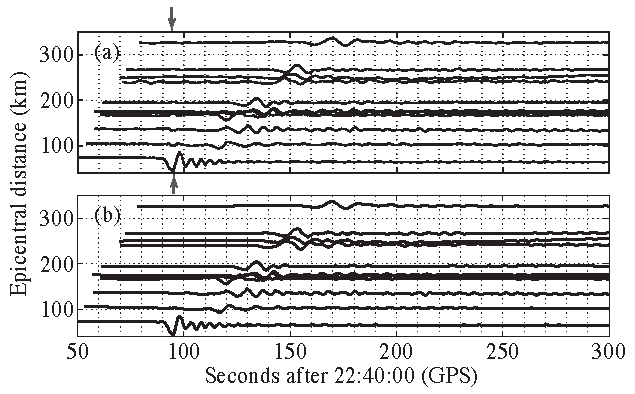
\includegraphics[width=0.99\linewidth]{./figures/ch2/fnoise_reduction.pdf}
    \caption[Noise reduction in CRTN stations with Kalman filtering]{Displacement waveforms in East component for (a) 1 Hz GPS only and (b) smoothed Kalman filter solutions for 12 collocated GPS/seismic stations in Southern California (Figure \ref{fig_mapelmayor}). Note the artifact (denoted by grey arrows) introduced by the GPS network adjustment at 95 seconds in (a) which is absent in (b), and the flatter (more precise) pre-event displacements in (b) compared to (a). All waveforms have been normalized for clarity. }
  \label{fig_noise_reduction}
\end{figure}

We note that there are certain limitations in the real-time estimation of displacements from GPS phase and pseudorange data. The introduction of very-high-rate precise accelerometer data at the GPS stations could help reduce the above problems in real-time applications by introducing independent confirmation of significant station displacement. For this purpose, a tightly coupled Kalman filter approach might be suitable \citep{Geng2013}. Instead of analyzing the already estimated GPS displacements with the raw accelerometer data, one could design a Kalman filter that instead uses the raw GPS phase and pseudorange observations and the raw accelerometer data, in order to improve the on-the-fly resolution of phase ambiguities. This is out of the scope of the present work \citep{Geng2013}. 
Finally station siting, monumentation, and mounting of GPS and seismic instruments at collocated stations is an important consideration. Seismic and geodetic networks developed independently and are seldom collocated. An interesting question for future consideration is whether costs can be reduced by using less sensitive and cheaper accelerometers (such as MEMS), or whether the current practice of installing high-end accelerometers in boreholes or shallow vaults is necessary. During a recent test (January 2014) at the LHPOST we evaluated low cost MEMS sensors which were collocated with observatory grade accelerometers. Analysis of this data should help answer this question in the future. \citet{evans2014} recently tested the performance of several low-cost sensors in the laboratory and found that while many of the very low cost ones are far from being useful for seismology many mid range ones seem to perform well enough for reliable strong motion sensing.

\section{Application to the $M_w$9 Tohoku-oki Earthquake}
\label{sec:tohoku}

One of the most relevant data sets for strong motions seismology in recent times is the set of records for the 2011 $M_w$9.0 Tohoku-oki earthquake. Complex waveforms with long durations of shaking recorded across dense geodetic and seismic networks make this an ideal test of the Kalman filter methodology. 

For this event we process data from 816 GPS stations throughout Honshu and Hokkaido Islands (Figure \ref{fig_map_tohoku}). As with the El Mayor-Cucuapah event we process the GPS data in a simulated real-time mode using the method of instantaneous positioning \citep{bock2000}. We triangulate the GPS network using a Delaunay triangulation scheme, and individual triangles are processed independently for relative station positions. The triangles are combined through a real-time network adjustment \citep{Crowell2009}, and station positions are referenced to station 0848 on Hokkaido Island, 900km northwest of the hypocenter (Figure \ref{fig_map_tohoku}). 

\begin{figure}[!ht] 
\centering
  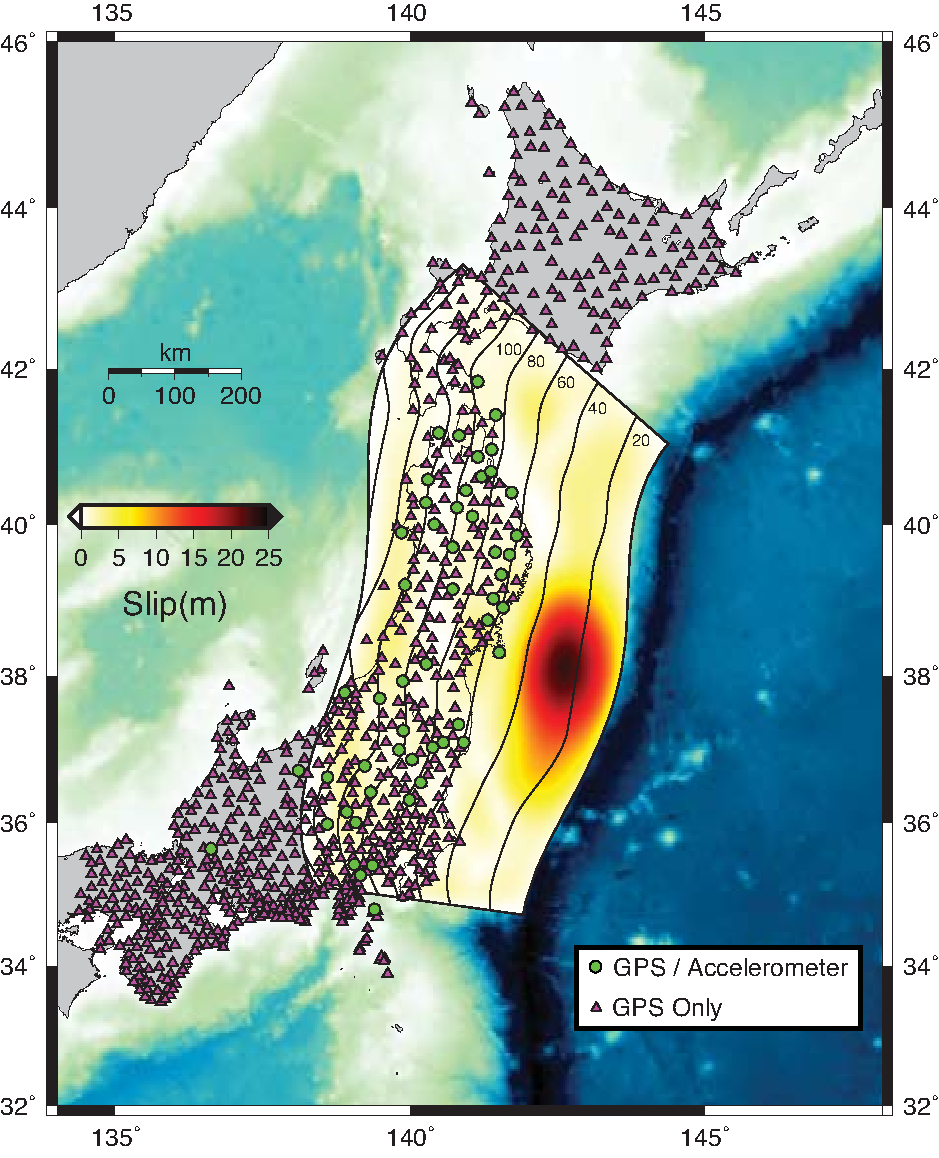
\includegraphics[width=0.85\linewidth]{./figures/ch2/map_tohoku.pdf}
    \caption[Collocated stations for the Tohoku-oki earthquake]{Station map depicting GPS only and GPS/accelerometer stations. Also included is the static slip inversion computed from real-time GPS (Chapter 3) and the iso-depth contours of the slab geometry determined in \citet{hayes2012}}
  \label{fig_map_tohoku}
\end{figure}

We identified 139 collocated GPS/accelerometer station throughout Japan. As before, we define a collocation as a pair of instruments separated by 1500m or less. Accelerometers in Japan function in triggered mode and many of those stations did not trigger in time. Furthermore, given the large duration of the source \citep{simons2011} many of those instruments terminated recording while significant shaking was ongoing. Thus, we culled the data set to 48 stations (Figure \ref{fig_map_tohoku}) that contain at least 2 seconds of pre-event noise and enough record to discern static offsets in the corrected data. Of these 48 stations 40 are K-net accelerometer sites and 8 are KiK-net accelerometer sites.

To establish a comparison with seismic-only data we compare the Kalman filtered displacements (KD) to baseline corrected data. We processed the 3 channel accelerometer data for those 48 stations using the method of \citet{Wang2011}. Recall from Section \ref{sec:strongmotion} that this method is an improvement over the BI correction scheme. The algorithm performs a grid search for the best correction parameters defining the optimal correction as that which best resembles a step function. This algorithm is presumed to be suitable for real-time computation because it requires no operator interaction. We also computed baseline corrections on the raw accelerometer data with the added constrain that the final waveform best fit the static offset from neighboring GPS station \citep{Wang2013}. Both of these variants are examples of Automated Baseline Correction (ABC).

For all three data sets, the automatic baseline corrections, the static field constrained baseline corrections and the Kalman filter we computed the power spectral density using the multi-taper method. We also computed 5\% damped displacement response spectra by finite difference solution to the single degree of freedom oscillator.

\subsection{Time Domain Analysis}

Figure \ref{fig_abc_nok} illustrates the results of ABC waveforms for 2 stations where no static field constrain has been applied. K-net station AOM011 is 296km from the event centroid and is an example of a station that is well corrected by the automated procedure. When compared to the KD waveform we see that the static offsets roughly match as does the shaking for all 3 components. In contrast K-net station GNM004, 430km from the centroid is an example of a failed correction. The displacement converges to the wrong value for the static field and as a result the shaking is also miscomputed. These two stations are the extremes of the behavior that we observe at the remaining stations.

\begin{figure}[!ht] 
\centering
  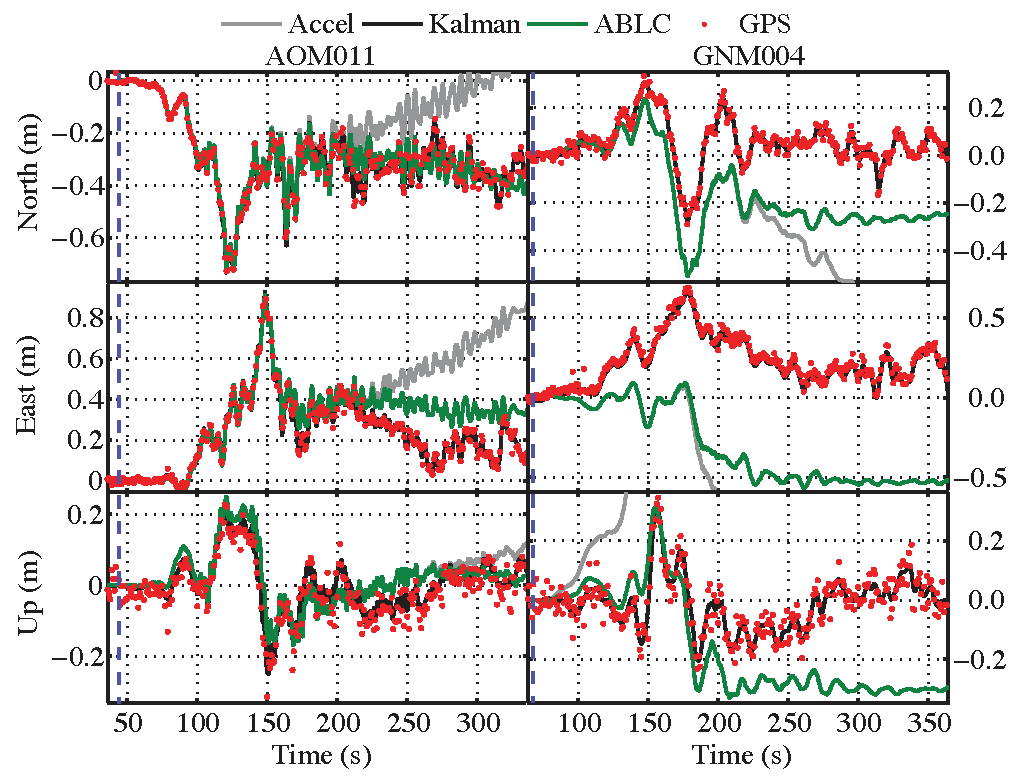
\includegraphics[width=0.99\linewidth]{./figures/ch2/abc_nok.pdf}
    \caption[Tohoku-oki baseline corrections with no constraints]{Results of applying the automatic baseline correction of \citet{Wang2011} with no static field constraints. The comparison is made to the Kalman filter, uncorrected accelerometer integration and 1 Hz GPS. K-net station AOM011 is 296 km from the centroid and K-net station GNM004 is 430 km from the centroid. The dotted line is the \textit{P} wave pick}
  \label{fig_abc_nok}
\end{figure}

As mentioned before we can apply the constrain that the ABC waveform converges to the static offset measured from a nearby GPS station. Figure \ref{fig_abc_withk} compares the result of applying such a constrain for K-net station AOM010, 323km from the centroid. This station is representative of the breadth of behavior we observe at all stations. The vertical channel fit to the KD waveform is greatly improved by adding the constraint. The east component is mildly improved but does not reach the level defined by the KD waveform. The improvement in the north component is only marginal and a large difference (20cm) remains in the static field between ABC and KD waveforms. Recall that we determine the optimum correction to be the one that best fits a step function of amplitude given by the static field. What these results indicate is that there might not be a combination of baseline correction times that provides a sufficient improvement to the displacement computation.

\begin{figure}[!ht] 
\centering
  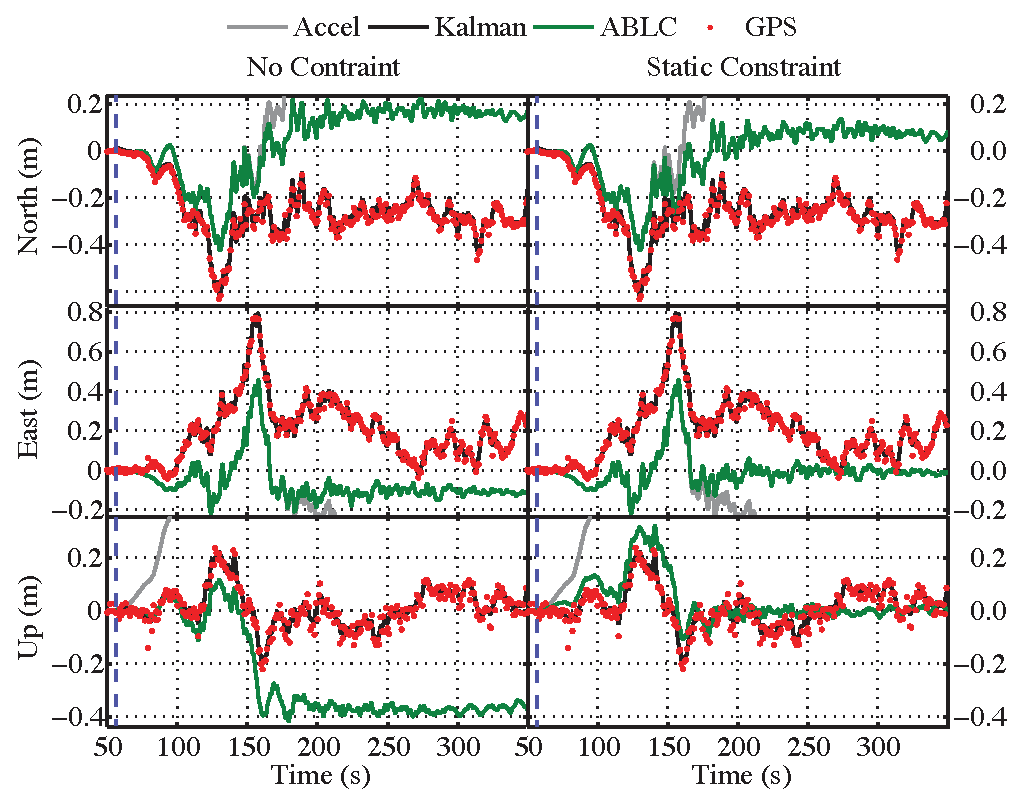
\includegraphics[width=0.99\linewidth]{./figures/ch2/abc_withk.pdf}
    \caption[Tohoku-oki baseline corrections with static field constraints]{Comparison between the ABC waveforms with and without the static field constraint. The results are for K-net station AOM010 323 km from the centroid and compared to the Kalman filter, uncorrected accelerometer integration and 1 Hz GPS. The dotted line is the \textit{P} wave pick}
  \label{fig_abc_withk}
\end{figure}

For both the constrained and unconstrained solutions there are records that compare favorably with the KD waveforms (Figures \ref{fig_abc_nok} and \ref{fig_abc_withk}). However, given the large amplitude motions present at most of these stations it is difficult to judge by simple visual inspection the adequacy of this comparison. Figure \ref{fig_abc_all} presents a record section with the difference between the KD waveforms and the ABC waveforms for all 48 stations ordered by distance to the centroid. We find that the difference is smallest in the earlier parts of the waveform. Additionally we see that the static field constrain improves the fit to the KD waveforms but large differences of several tens of centimeters remain. Also notice that the stations closest to the centroid are the ones with the poorest fits that even with the addition of the static field constrain improve little.

\begin{figure}[!ht] 
\centering
  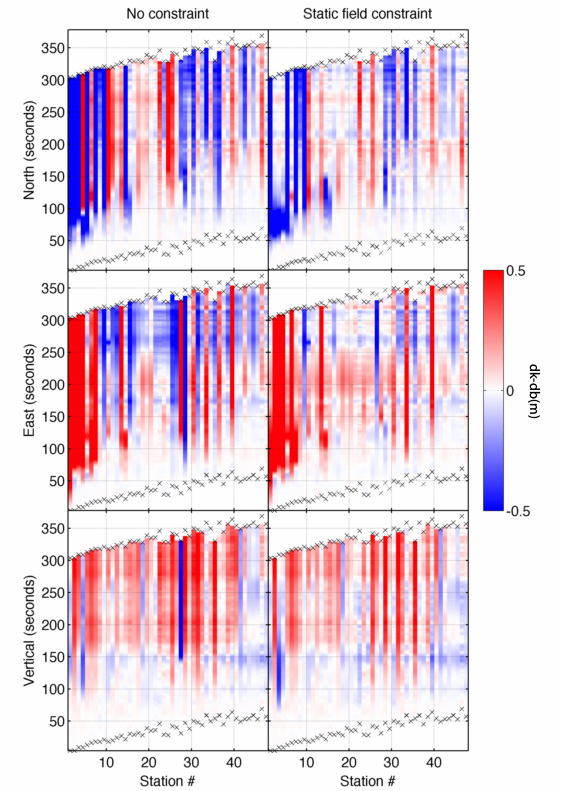
\includegraphics[width=0.65\linewidth]{./figures/ch2/abc_all.jpg}
    \caption[Tohoku-oki Kalman filter performance at 48 stations]{Difference between the KD and ABC waveforms for both constrained and unconstrained solutions. The stations are ordered by increasing distance to the centroid and the crosses denote the start and end of each waveform.}
  \label{fig_abc_all}
\end{figure}

Inspection of the KD waveforms (Figures \ref{fig_abc_nok} and \ref{fig_abc_withk})  shows that the Kalman filter method corrects the 3 components of motion at all 48 stations successfully. We decimate the KD and ABC static field constrained waveforms to the GPS sample times and compute the RMS of the difference between both sets of waveforms and the GPS (Figure \ref{fig_abc_rms}). In the north direction the RMS for the ABC waveforms ranges from 4.3 cm to 150 cm, for the KD waveforms the range is from 0.6cm to 5cm. In the east direction, the ABC waveforms have RMS values from 6 cm to 320 cm and the KD waveforms from 1cm to 10cm. In the vertical direction the ABC waveforms have RMS values that range from 4cm to 43cm and the KD waveforms from 2cm to 10cm. For all stations on all channels we find that the KD waveforms have a smaller RMS than the ABC waveforms.

\begin{figure}[!ht] 
\centering
  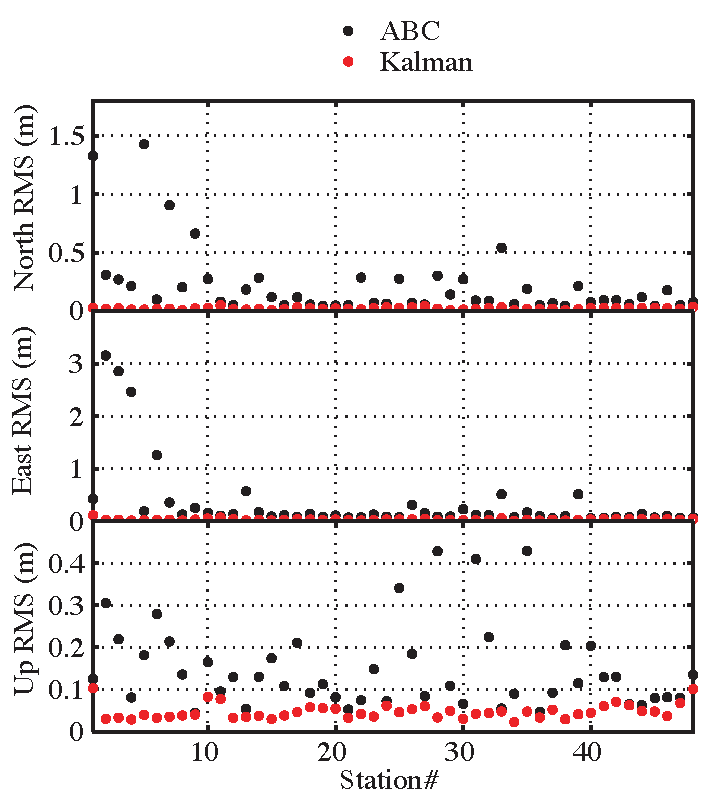
\includegraphics[width=0.7\linewidth]{./figures/ch2/abc_rms.pdf}
    \caption[RMS between baseline corrections and Kalman filtered waveforms]{RMS of the difference between the ABC and GPS waveforms and the KD and GPS waveforms for all stations. The stations are ordered by increasing distance from the centroid.}
  \label{fig_abc_rms}
\end{figure}

\subsection{Frequency Domain Analysis}

It remains unclear at which frequencies baseline corrections introduce errors into measurements. This is of consequence for source observations and strong motion analysis. Also, it is generally assumed that baseline corrections have no effect at frequencies of engineering interest \citep{Boore2001,Boore2005}. In the following is a frequency domain analysis where we compare ABC and KD waveforms.

Figure \ref{fig_abc_psd} is an example of the power spectral density (PSD) for ABC, KD, uncorrected accelerometer integration and GPS data for the north component of K-net station AOM027, 363km from the centroid. These results are for the unconstrained baseline correction. The results are consistent with Section \ref{sec:proof}, namely that the accelerometer over estimates long period content and that GPS overestimates the spectral content at the higher end of its frequency band. Furthermore one can observe the desirable characteristics of the KD waveforms; they follow the GPS spectra at low frequencies and transition to the accelerometer at high frequencies. It is also interesting to note that the ABC waveform has different frequency content than the KD waveforms at frequencies at least as high as 0.5Hz and that the ABC waveform does not agree with the GPS at any part of the long period spectrum.

\begin{figure}[!ht] 
\centering
  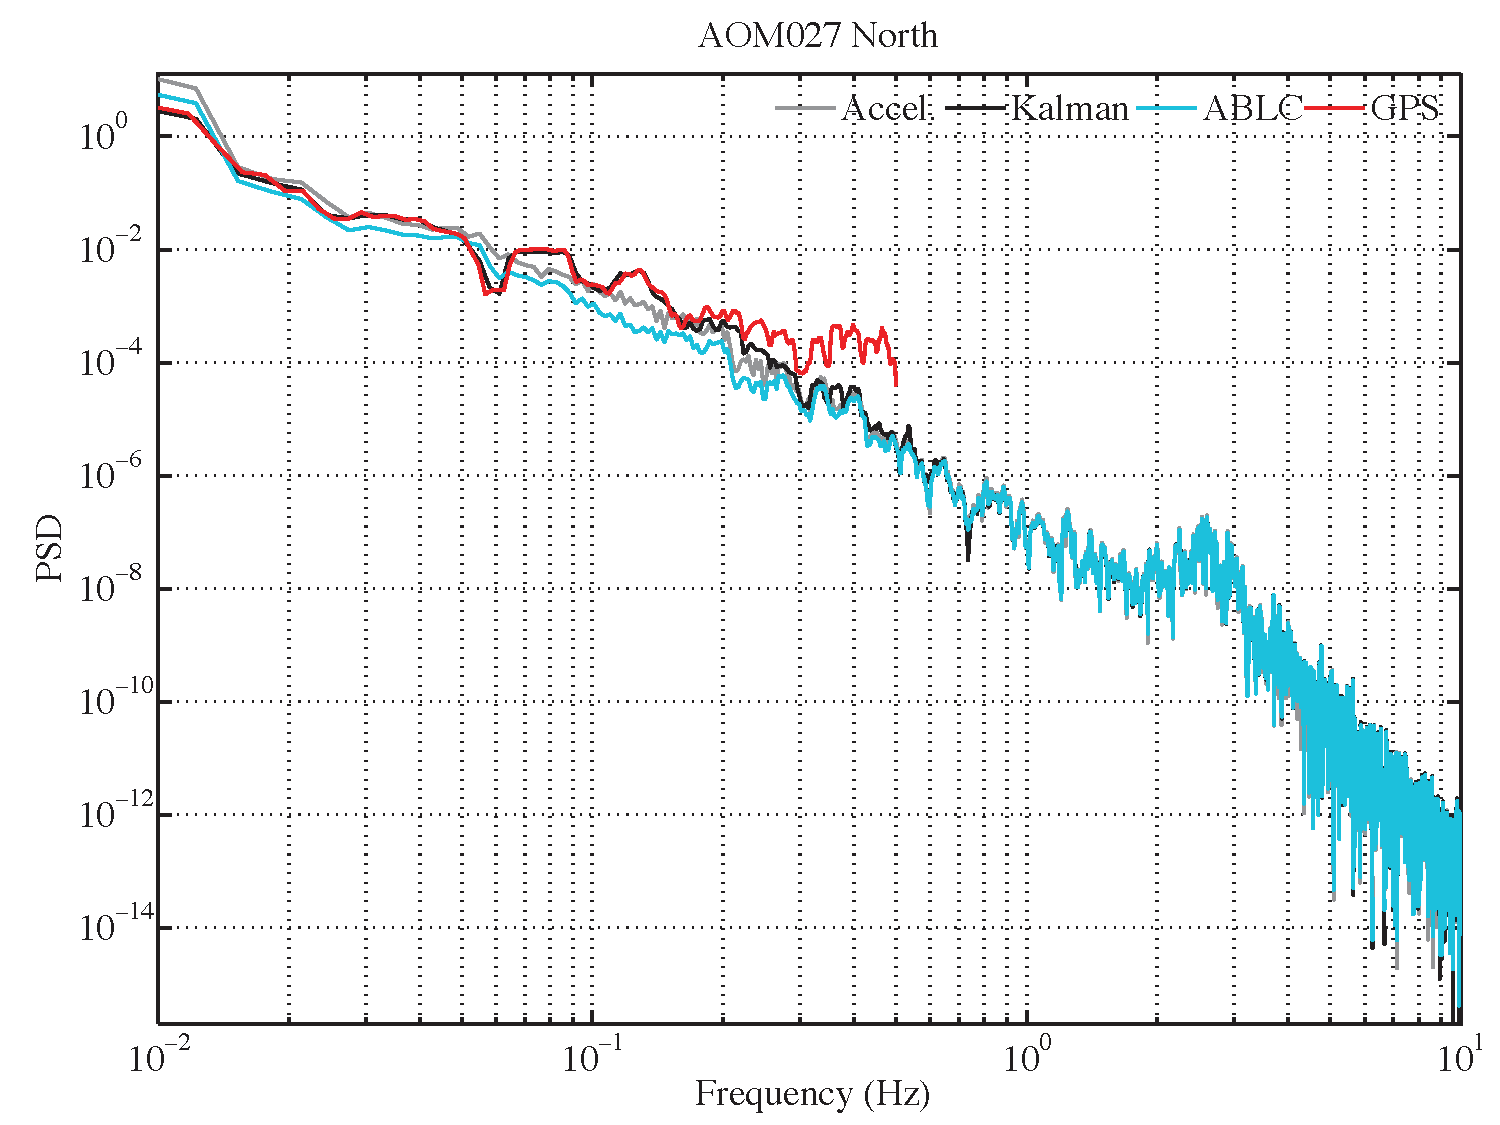
\includegraphics[width=0.82\linewidth]{./figures/ch2/abc_psd.pdf}
    \caption[PSD of baseline corrected and Kalman filtered data]{Power spectral densities for the north displacements at K-net station AOM027, 363 km from the centroid. These results are for the unconstrained baseline correction.}
  \label{fig_abc_psd}
\end{figure}

Figure \ref{fig_abc_respspec} is a similar analysis for the displacement response spectra. The results are for the east component of station K-net station MYG001 138km from the centroid. The ABC solution is unconstrained. In line with the PSD analysis, we find that the KD waveform tracks the GPS result at long periods and the uncorrected accelerometer at high frequencies. Similarly we find that the uncorrected accelerometer spectrum differs from the KD result at periods longer than ~11s while the ABC spectrum begins to diverge from the KD spectrum at around ~13s. It is also important to note that for periods shorter than 10s the GPS only spectrum is unreliable.

\begin{figure}[!ht] 
\centering
  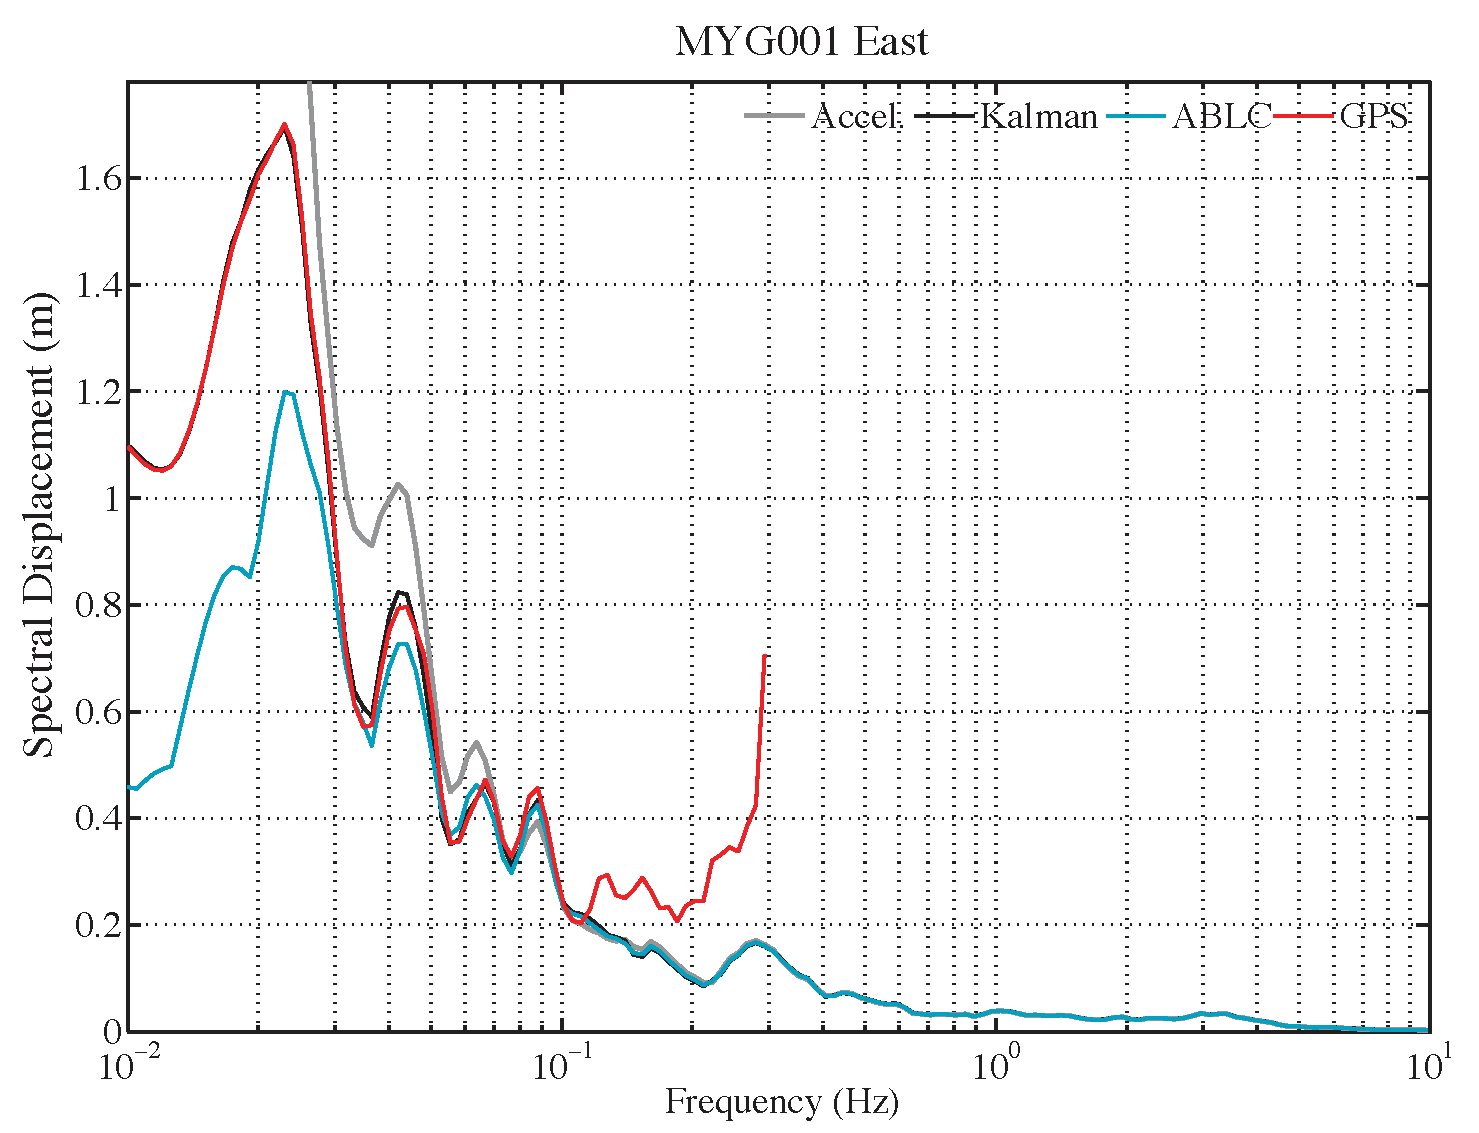
\includegraphics[width=0.82\linewidth]{./figures/ch2/abc_respspec.pdf}
    \caption[Response spectra of baseline corrected and Kalman filtered data]{5\% damped displacement response spectra for the east component of K-net station MYG001 138km from the centroid. These results are for the unconstrained baseline correction.}
  \label{fig_abc_respspec}
\end{figure}

To better understand the relationship between the ABC and KD PSDs we computed the ratio between the KD PSDs and ABC PSDs for all stations. This is shown in logarithmic scale in Figure \ref{fig_abc_psdall} for both the constrained and unconstrained corrections and ordered by distance to the centroid. Several features are of interest, first that the discrepancy between the KD and ABC spectra are larger for stations close to the source. At long periods there is mixed behavior between over and under estimation of the spectra by the ABC results in the horizontal components. However, for the vertical component we find that the ABC spectra consistently overestimate the frequency content. It is also important to note that the differences in spectral content are of consequence for frequencies as high as 0.5 Hz. We also find that addition of the static field constrain provides only a marginal improvement in the estimation at long periods. Addition of this constrain leads to little to no improvement in the recovery of the mid-range frequencies.

\begin{figure}[!ht] 
\centering
  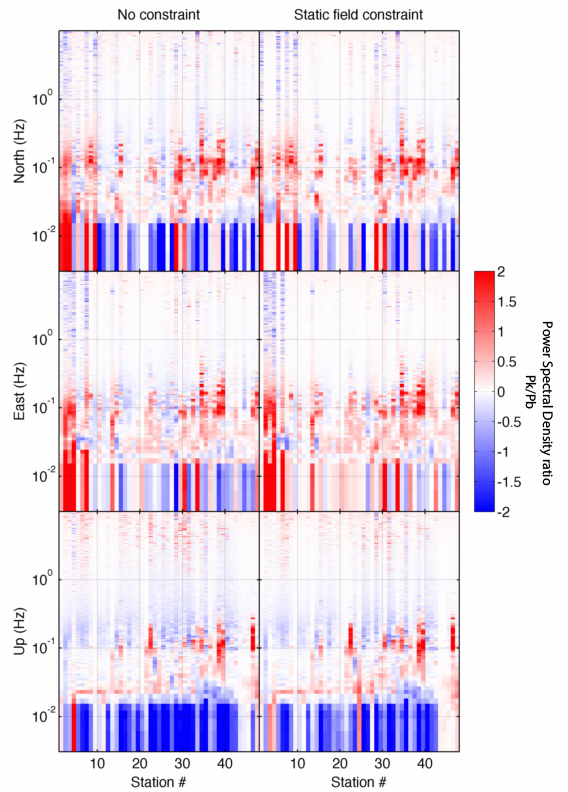
\includegraphics[width=0.75\linewidth]{./figures/ch2/abc_psdall.jpg}
    \caption[PSD ratios for collocated sites]{Logarithm of the ratio between the KD and ABC power spectra for all stations ordered by increasing distance to the centroid. Results are for both constrained and unconstrained waveforms.}
  \label{fig_abc_psdall}
\end{figure}

Figure \ref{fig_abc_respspecall} is a similar plot for the response spectra, here we present the difference between the KD and ABC derived spectral displacements for both constrained and unconstrained results. Similar to what we described for the PSD comparison, we find a better fit by the ABC spectra in the vertical direction than in the horizontal directions. Additionally we find little improvement in the spectral displacement estimates from addition of the static field constraint. We also find that for the response spectra the largest differences occur at periods longer than 8-9s.

\begin{figure}[!ht] 
\centering
  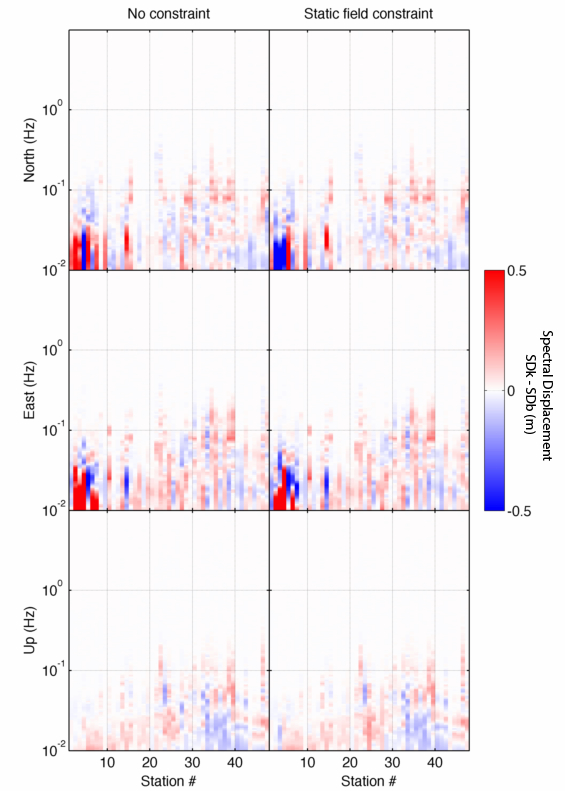
\includegraphics[width=0.75\linewidth]{./figures/ch2/abc_respspecall.jpg}
    \caption[Response spectra difference for collocated sites]{Difference between the KD and ABC 5\% damped response spectra for all stations ordered by increasing distance to the centroid. Results are for both constrained and unconstrained waveforms.}
     \label{fig_abc_respspecall}
\end{figure}

\subsection{Performance of the Filter and Prospects for Automated Baseline Corrections}

Even though GPS has higher noise levels and aliasing effects are present, whatever method is chosen to compute the displacements (KD or ABC) it must agree broadly with the GPS time series. Figures \ref{fig_abc_nok}-\ref{fig_abc_all} demonstrate this and show that with the Kalman filter we achieve accurate recovery of both permanent and transient motions while serious difficulties arise when employing the ABC method. We assert that this verifies that the Kalman filter methodology described in Section \ref{sec:kalman} has no substantive problems in resolving broadband displacements for the $M_w$9.0 Tohoku-oki earthquake. That we have done so using the K-net acceleration data is important. As acknowledged by \citet{Wang2013} recovery of displacements from those records is difficult because of the large baseline offsets, ostensibly introduced because of unfavorable site conditions. The incorporation of real-time GPS with the Kalman filter resolves these offsets with little difficulty.

However, we recognize that collocation of GPS and strong motion sensors are still the exception rather than the norm, and baseline corrected displacements are important. We have evaluated the suitability of automated baseline correction procedures in both the time and frequency domain. We independently verified that automatic baseline correction schemes such as that of \citet{Wang2011} can indeed produce in some cases waveforms that accurately capture both static and dynamic motions. However for the subset of 48 stations we found that there can be very large differences in the estimated static offsets when compared to actual offsets measured by the real-time GPS (Figure \ref{fig_abc_map_offsets}). This is important because as previously discussed current areas of research for rapid earthquake response include modeling of the source with static offsets. If the offsets determined from the ABC scheme are unreliable their utility for rapid response will be very limited.  \citet{Wang2013} proposed detecting outliers in the static field estimation by comparison with synthetics determined from a static slip inversion. This necessitates some important assumptions, for example for 2011 Tokachi-oki that the earthquake has ruptured the mega-thrust and that the mechanism is reverse faulting. These assumptions are critical and will not always hold up. Outer rise normal faulting events can be sizeable and are not uncommon. Large strike slip events close to the trench such as the $M_w$8.6 strike-slip event Wharton Basin off Sumatra, Indonesia on 11 April 2012 \citep{satriano2012} will be significantly mis-modeled. Furthermore quiescent borehole stations such as those of the KiK-net deployment used in \citet{Wang2013} are not the norm. Rather, stations of heterogeneous site response like those of the K-net deployment are more common in networks worldwide.

\begin{figure}[!ht] 
\centering
  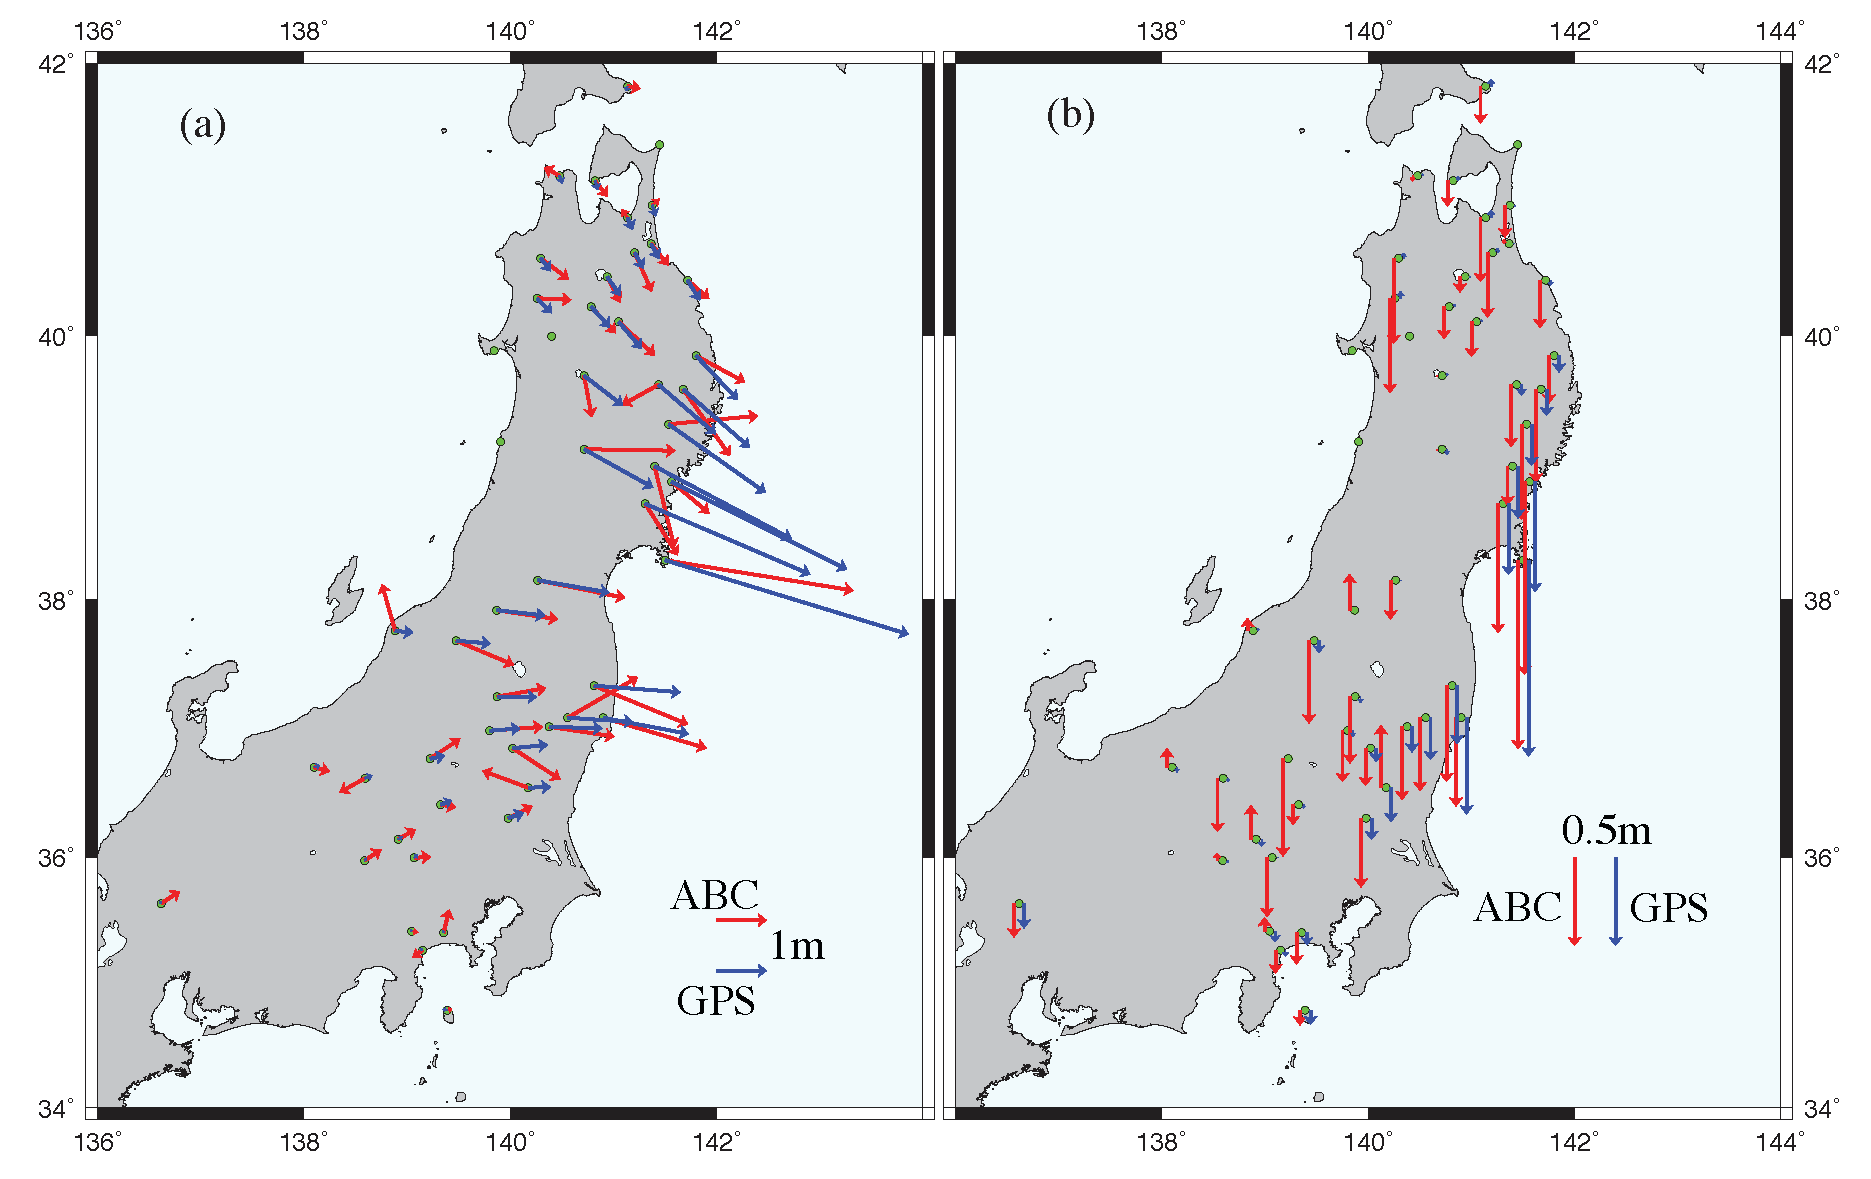
\includegraphics[width=0.99\linewidth]{./figures/ch2/abc_map_offsets.pdf}
    \caption[Coseismic offset comparisson]{Comparison between static offsets determined from the automated baseline corrected procedure and the real-time GPS. (a) Are horizontal and (b) are vertical offsets}
     \label{fig_abc_map_offsets}
\end{figure}

We have identified important discrepancies between ABC and KD waveforms. The automatic corrections can converge to solutions that look plausible but as shown in Figure \ref{fig_abc_nok} can be very far from the correct solution. Even with addition of the static field constrain the baseline offsets might be so large that the simple bilinear scheme is not enough to correct the data. But the most troubling case is shown in Figure \ref{fig_abc_bad}. This presents the north component of K-net station IWT009 157km from the centroid and corrected with the static offset constraint. The plot shows that the ABC waveform converges to the correct static value but the shaking is miscomputed by as much as 0.5m. This type of behavior is not uncommon in the corrections. Thus, the assumption that convergence to the static field value ensures reliability of the waveform is not routinely satisfied. It is possible for a correct static field to be computed but to be in error by large amounts in the dynamic component of the waveform.

\begin{figure}[!ht] 
\centering
  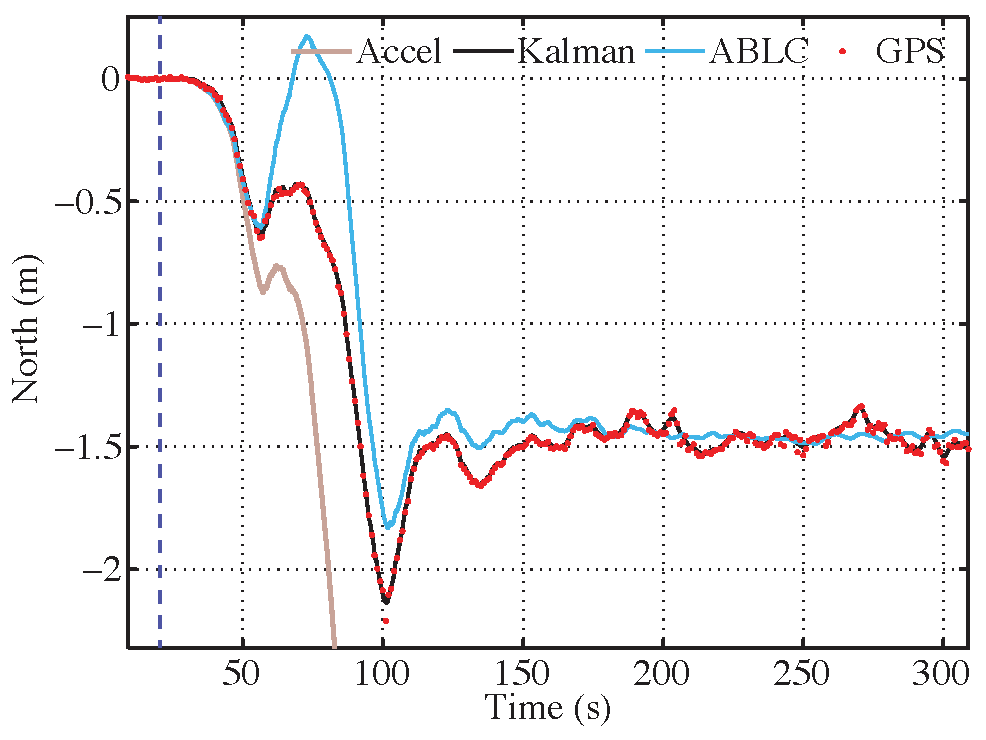
\includegraphics[width=0.7\linewidth]{./figures/ch2/abc_bad.pdf}
    \caption[Example of failed correction at station IWT009]{North displacement waveforms for station K-net station IWT009 157 km from the centroid.}
     \label{fig_abc_bad}
\end{figure}

We too find that addition of the static field constrained as proposed by \citet{Wang2013} improves the time domain solution. Nonetheless we have also shown that ABC waveforms even when they converge to the correct static offset value can still be in error in regards to the transient component of the waveform (Figure \ref{fig_abc_bad}).

The frequency domain analysis also shows some interesting behavior. We have once again demonstrated the performance of the Kalman filter displacements, following the GPS spectra at long periods and the accelerometer spectra at higher frequencies. We have also shown that the ABC PSD can be miscomputed at frequencies as high as $\sim$0.5Hz. Furthermore we have demonstrated that addition of the static field constrain does little to improve the spectral recovery.

With the response spectra we have found a similar pattern except that the ABC spectra incurred in an error at lower frequencies, usually at periods longer than 8-9s. These discrepancies in both PSD and response spectra are well within the frequencies that are of interest to engineering seismology, especially for the PSD estimation. Furthermore the frequency domain error incurred by the ABC waveforms is not simple. Sometimes it is an overestimate and sometimes an underestimate. This has relevance for seismological applications that seek to use baseline corrected waveforms for strong ground motion analysis, source studies and response. This is true as well for engineering purposes. \citet{Boore2002} had already shown that this might be the case but found that for most stations the bias was introduced at much longer periods. However, that conclusion was reached from accelerometer data alone and no comparison was made to the frequency content of high rate GPS or combined data, which was unavailable at the time.
Tangentially we have demonstrated that the useful frequency content of GPS-only waveforms is also limited to periods longer than 10 s. Higher-frequency studies from high rate data will be impeded by over estimates of the spectral content.

If indeed rotational motions account for most of the baseline offsets, and this seems to be the case \citep{Trifunac2001,Graizer2006}, then aspiring to design an algorithm that can accurately and objectively correct acceleration from acceleration data alone is a frustrating proposition. There is no way to simply distinguish between rotations and translations with enough sensitivity from the inertial sensor itself. Furthermore, although the incorporation of outside constraints, such as the static field, improves matters it does not solve the problem. For a simple waveform with short duration and small accelerations, incorporating the static constrain might suffice. However for the Tohoku-oki waveforms, which have complex shapes, this simple constrain is insufficient. Rotational motions happen continuously throughout the record and introduce baseline offsets of different amplitudes in a continuous fashion, not in the simple piecewise manner in which we have traditionally tried to model them. Thus constraining the end of the record is not enough and there is no way to objectively determine offsets that happen earlier in the record

The aggregate of results and analysis we show here is by no means proof by exhaustion of the unsuitability of automatic baseline corrections. Other schemes might yet be developed that provide better results. However we have shown that the corrections in this particular case are suspect for static field determination; that they might miscompute the dynamic component of the seismogram and that the errors are incurred at frequencies well within what is of interest to seismology and engineering. Furthermore, we have shown that broadband displacements computed from collocated GPS and accelerometers via a Kalman filter have none of those problems.

While collocations are still not the norm, this work as well as that of \citet{Wang2013} argue that low-cost micro electro-mechanical sensors (MEMS) are increasingly desirable for regional monitoring. MEMS accelerometers are a fraction of the cost of observatory grade accelerometers. Thus, given the current limitations of baseline correction procedures, the superior performance of collocated processing techniques and the availability of cheaper sensors we advocate that if broadband displacements are a priority target of a particular network, then retrofitting of existing geodetic infrastructure with accelerometers should be given a high priority. We find it unlikely that displacements from accelerometer data alone will reach the robustness or reliability required for real-time and rapid observations.

%\appendix
%\chapter{Final notes}
%  Remove me in case of abdominal pain.

